\section{Partial Zipping}\label{ap:partial_zipping}
In Fig.~\ref{fig:varying_partial_zip} we plot the average per task accuracy by the number of layers zipped in ResNet-20$\times$8 for CIFAR-100 (50+50) and ResNet-50 for ImageNet-1k (200+200). 
Note that to avoid adding extra unmerge modules into the network, our stopping point while unzipping has to be the end of a stage. 

In Table~\ref{tab:partialzip_corrs}, we show the average neuron correlations at each partial-zipping stage between the layers of ResNet-20 ($8\times$) models trained on the CIFAR-100 (50+50) task. 
We collect results using the same models used in Table \ref{tab:cifar50+50}, and compute correlations as described in Section \ref{sec:approach}.
Overall, we find the correlations between models consistently decreases through successive partial zipping locations. 
This corroborates the finding of \citet{kornblith2019similarity} that model layers become increasingly dissimilar with depth, as they encode more task-specific features. 
Coupling Table \ref{tab:partialzip_corrs} with Figure \ref{fig:partial_zip_cifar100}, we observe a direct correlation between layer-(dis)similarities and performance decrease.
This illustrates the importance of layer similarity between two networks and strong performance.
% \begin{figure}[t]
% \centering

% \subfloat[
%     \textbf{CIFAR-100 50+50.}
%     \label{fig:partial_zip_cifar100}
% ]{
% \centering
% \begin{minipage}{0.49\linewidth}{
% \begin{center}
%     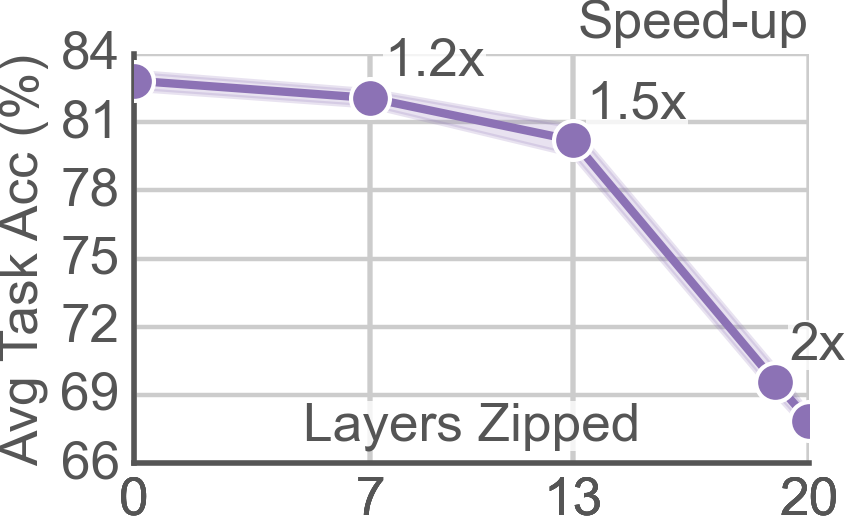
\includegraphics[width=\linewidth]{figures/imgs/partial_zip_CIFAR_50_50.png}
% \end{center}
% }\end{minipage}
% }
% \subfloat[
%     \textbf{ImageNet-1k 200+200.}
%     \label{fig:partial_zip_imagenet}
% ]{
% \centering
% \begin{minipage}{0.49\linewidth}{
% \begin{center}
%     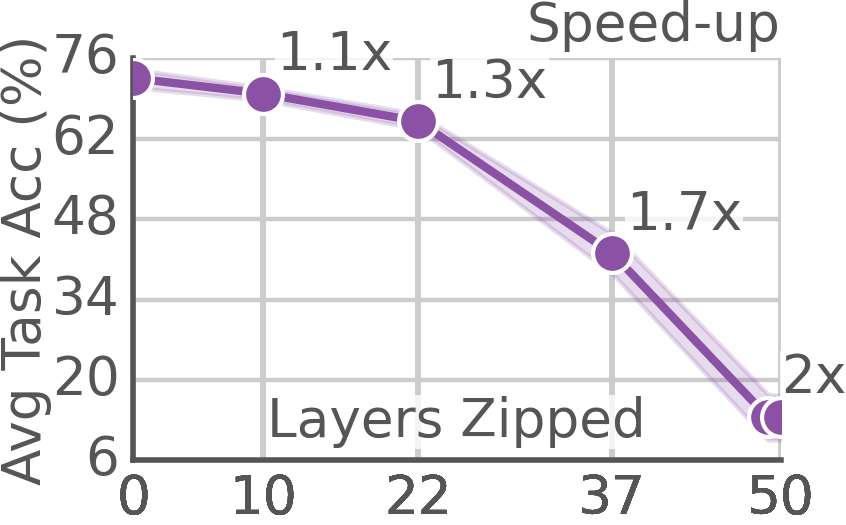
\includegraphics[width=\linewidth]{figures/imgs/partial_zip_imnet_200_200.png}
% \end{center}
% }\end{minipage}
% }

% \caption{
% {\bf Varying Partial Zip.} 
% By leaving some layers unzipped (Sec.~\ref{sec:partial_zip}), we can recover a significant amount of performance while still merging most of the model. 
% }
% \label{fig:varying_partial_zip}
% \end{figure}

% \begin{wrapfigure}{r}{0.48\linewidth}
% \vspace{-10pt}
% \centering
% \resizebox{\linewidth}{!}{
%     \tablestyle{5pt}{1.1}
%     {
%     \tablestyle{5pt}{1.1}
%     \begin{tabular}{x{40}x{40}x{40}}
%         \multicolumn{3}{c}{Average Stage Correlations}\\
%         Layer \sfrac{7}{20} & Layer \sfrac{13}{20} & Layer \sfrac{19}{20}\\
%     \shline
%     {0.50\conf{0.01}} & {0.37\conf{0.00}} & {0.27\conf{0.00}} \\
%     \hline
% \end{tabular}
%     }
% }
% \captionof{table}{\textbf{CIFAR-100 (50+50) Zipping Correlations.} We show the average correlations between two ResNet-20 ($8\times$) models at each partial zipping stage. Correlations consistently decrease at each successive stage, indicating that the layers of the two models increasingly diverge. 
% }
% \label{tab:partialzip_corrs}
% % \end{table}
% \vspace{-20pt}
% \end{wrapfigure}


\begin{wrapfigure}{r}{0.48\linewidth}
\vspace{-15pt}
\begin{minipage}[l]{\linewidth}{
\captionsetup{justification=centering}
\subfloat[
    \textbf{CIFAR-100 \\ \ \ \ \ (50+50)}
    \label{fig:partial_zip_cifar100}
]{
\centering
\begin{minipage}{0.48\linewidth}{
\begin{center}
    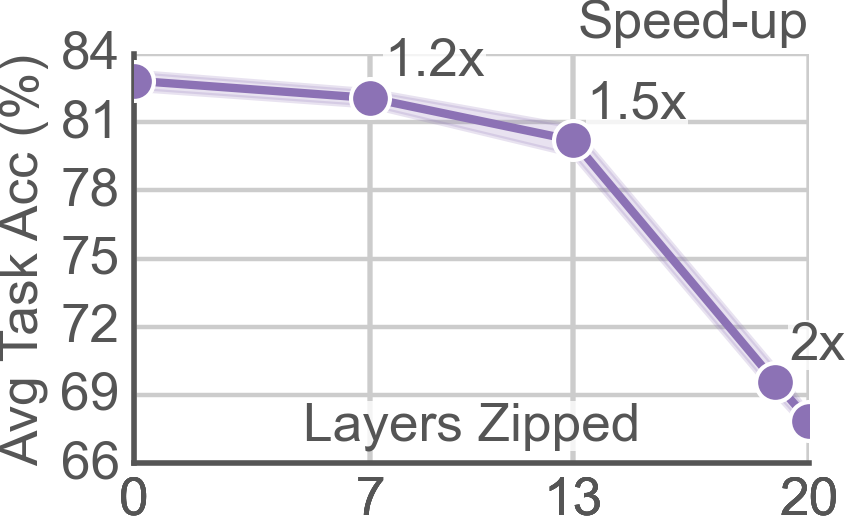
\includegraphics[width=\linewidth]{figures/imgs/partial_zip_CIFAR_50_50.png}
\end{center}
}\end{minipage}
}
\subfloat[
    \textbf{ImageNet-1k \\ \ \ \  (200+200)}
    \label{fig:partial_zip_imagenet}
]{
\centering
\begin{minipage}{0.48\linewidth}{
\begin{center}
    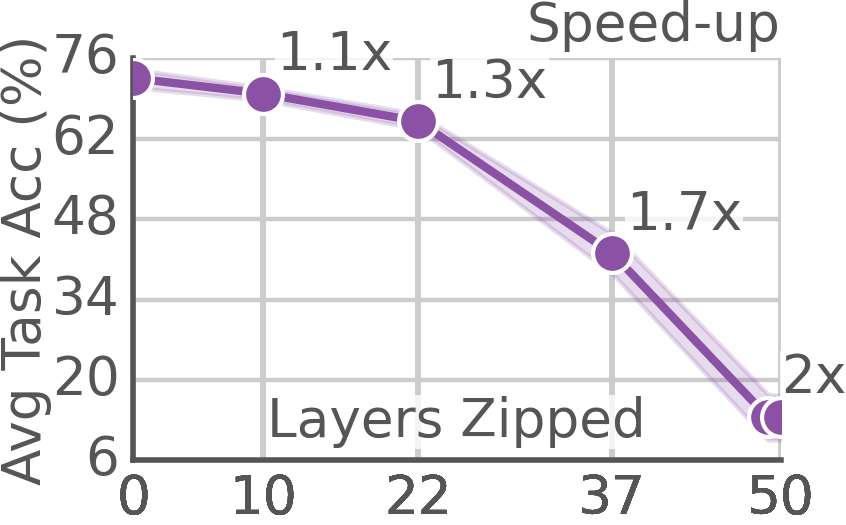
\includegraphics[width=\linewidth]{figures/imgs/partial_zip_imnet_200_200.png}
\end{center}
}\end{minipage}
}
\captionsetup{justification=justified}
        \caption{{\bf Varying Partial Zip.} By leaving some layers unzipped (Sec.~\ref{sec:partial_zip}), we can recover a significant amount of performance while still merging most of the model. }
\label{fig:varying_partial_zip}
}\end{minipage}
\begin{minipage}[l]{\linewidth}{
\vspace{5pt}
\centering
\resizebox{\linewidth}{!}{
    \tablestyle{5pt}{1.1}
    {
    \tablestyle{5pt}{1.1}
    \begin{tabular}{x{40}x{40}x{40}}
        \multicolumn{3}{c}{Average Stage Correlations}\\
        Layer \sfrac{7}{20} & Layer \sfrac{13}{20} & Layer \sfrac{19}{20}\\
    \shline
    {0.50\conf{0.01}} & {0.37\conf{0.00}} & {0.27\conf{0.00}} \\
    \hline
\end{tabular}
    }
}
\captionof{table}{\textbf{CIFAR-100 (50+50) Zipping Correlations.} We show the average correlations between two ResNet-20 ($8\times$ width) models at each partial zipping stage. Correlations consistently decrease at each successive stage, indicating that the layers of the two models increasingly diverge. 
}
\label{tab:partialzip_corrs}
% \end{table}
% \vspace{10pt}
}\end{minipage}
\begin{minipage}[l]{\linewidth}{
\captionsetup{justification=centering}
\vspace{1em}
\subfloat[
    \textbf{CIFAR-100 \\ \ \ \ \ (50+50)}
    \label{fig:data_use_cifar100}
]{
\centering
\begin{minipage}{0.48\linewidth}{
\begin{center}
    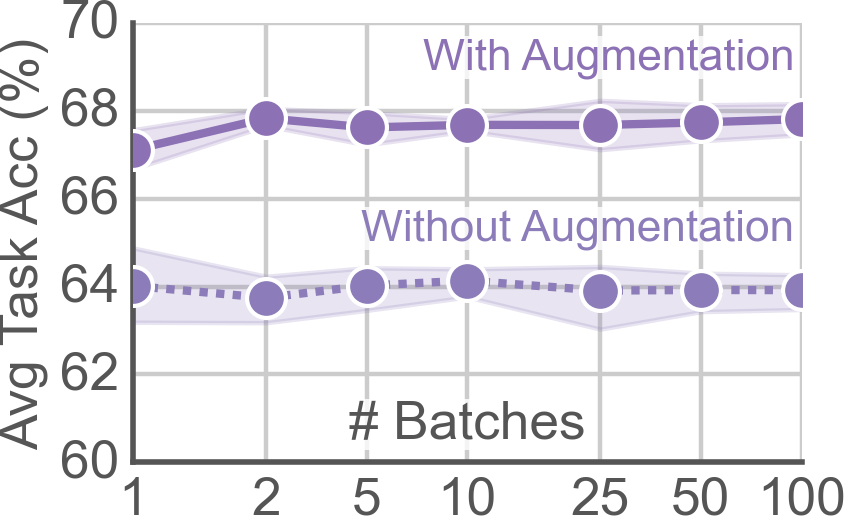
\includegraphics[width=\linewidth]{figures/imgs/cifar100_data.png}
\end{center}
}\end{minipage}
}
\subfloat[
    \textbf{ImageNet-1k \\ \ \ \  (200+200)}
    \label{fig:data_use_imagenet}
]{
\centering
\begin{minipage}{0.48\linewidth}{
\begin{center}
    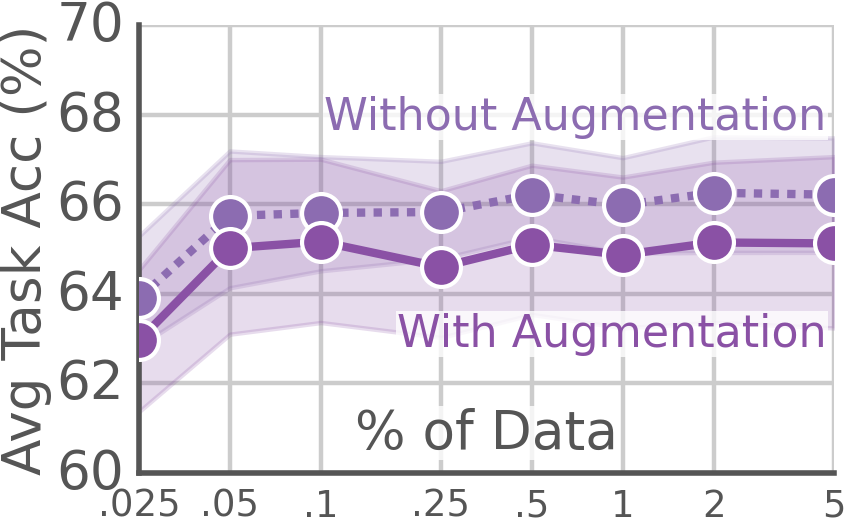
\includegraphics[width=\linewidth]{figures/imgs/imnet200_data.png}
\end{center}
}\end{minipage}
}
\captionsetup{justification=justified}
\caption{
{\bf Data Usage.} 
How much data do we need to use to compute activations? 
We find that only a few hundred images are needed to obtain the best performance.
Data augmentation is not always useful.
% Here we ablate the amount of data used for our CIFAR-100 (50+50) ResNet-20 ($8\times$ width) and ImageNet (200+200) Resnet-50 (\sfrac{22}{50} layers) experiments. 
% The batch size used is 500 for CIFAR and 16 for ImageNet. 
% In both cases, we only need a few hundred images to obtain the best results. 
% On the other hand, data augmentation is necessary for CIFAR but hurts for ImageNet. Our default for all experiments uses data augmentation and the full set for CIFAR (100 batches) and 1\% of the data for ImageNet. 
}
\label{fig:data_usage}
}\end{minipage}
% \vspace{-60pt}
\end{wrapfigure}

% \begin{wrapfigure}{l}{0.52\linewidth}
% % \vspace{-260pt}
% \begin{minipage}[l]{\linewidth}{
% \subfloat[
%     \textbf{CIFAR-100 (50+50).}
%     \label{fig:data_use_cifar100}
% ]{
% \centering
% \begin{minipage}{0.48\linewidth}{
% \begin{center}
%     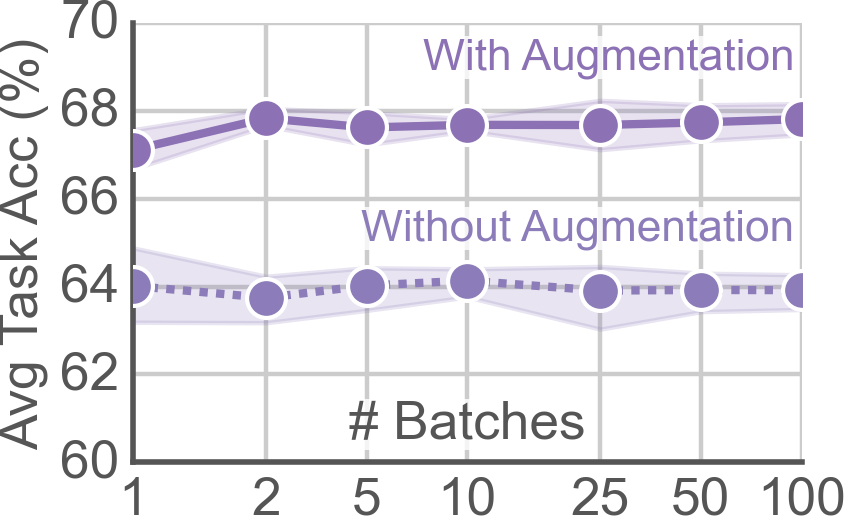
\includegraphics[width=\linewidth]{figures/imgs/cifar100_data.png}
% \end{center}
% }\end{minipage}
% }
% \subfloat[
%     \textbf{ImageNet-1k (200+200).}
%     \label{fig:data_use_imagenet}
% ]{
% \centering
% \begin{minipage}{0.48\linewidth}{
% \begin{center}
%     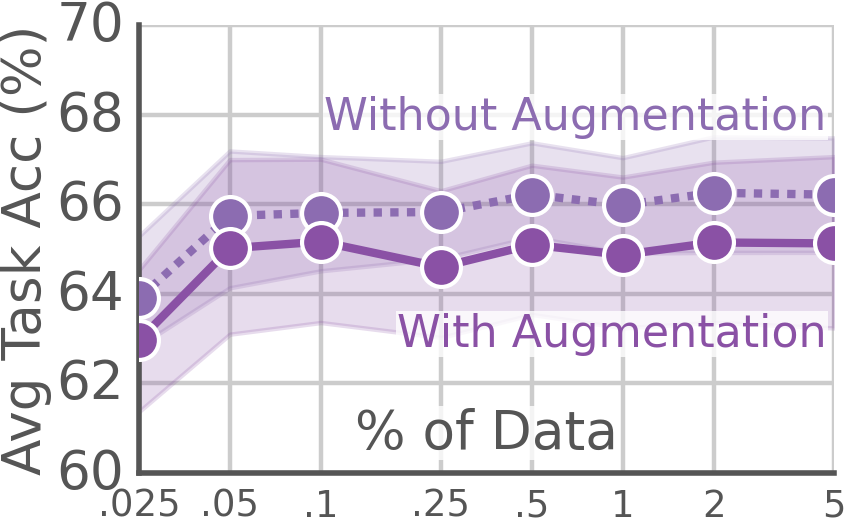
\includegraphics[width=\linewidth]{figures/imgs/imnet200_data.png}
% \end{center}
% }\end{minipage}
% }
%         \caption{
%         {\bf Data Usage.} How much data do we need to use to compute activations? Here we ablate the amount of data used for our CIFAR-100 (50+50) ResNet-20 ($8\times$ width) and ImageNet (200+200) Resnet-50 (\sfrac{22}{50} layers) experiments. The batch size used is 500 for CIFAR and 16 for ImageNet. In both cases, we only need a few hundred images to obtain the best results. On the other hand, data augmentation is necessary for CIFAR but hurts for ImageNet. Our default for all experiments uses data augmentation and the full set for CIFAR (100 batches) and 1\% of the data for ImageNet. 
%         }
% \label{fig:data_usage}
% }\end{minipage}
% \end{wrapfigure}


% \caption{{\bf Data Usage.} How much data do we need to use to compute activations? Here we ablate the amount of data used for our CIFAR-100 (50+50) ResNet-20 ($8\times$ width) and ImageNet (200+200) Resnet-50 (\sfrac{22}{50} layers) experiments. The batch size used is 500 for CIFAR and 16 for ImageNet. In both cases, we only need a few hundred images to obtain the best results. On the other hand, data augmentation is necessary for CIFAR but hurts for ImageNet. Our default for all experiments uses data augmentation and the full set for CIFAR (100 batches) and 1\% of the data for ImageNet. }
% \label{fig:data_usage}
% \end{figure}


% \begin{figure}
%     \begin{minipage}[t]{0.50\linewidth}
%         \centering
%         \subfloat[
%             \textbf{CIFAR-100 (50+50).}
%             \label{fig:partial_zip_cifar100}
%         ]{
%             \centering
%             \begin{minipage}{0.40\linewidth}{
%                 \centering
%                 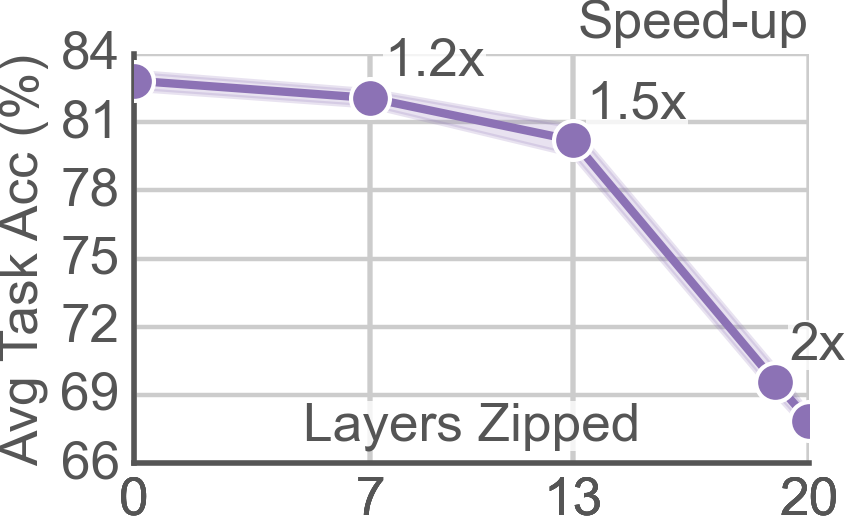
\includegraphics[width=\linewidth]{figures/imgs/partial_zip_CIFAR_50_50.png}
%             }\end{minipage}
%         }
%         \subfloat[
%             \textbf{ImageNet-1k (200+200).}
%             \label{fig:partial_zip_imagenet}
%         ]{
%             \centering
%             \begin{minipage}{0.40\linewidth}{
%                 \centering
%                 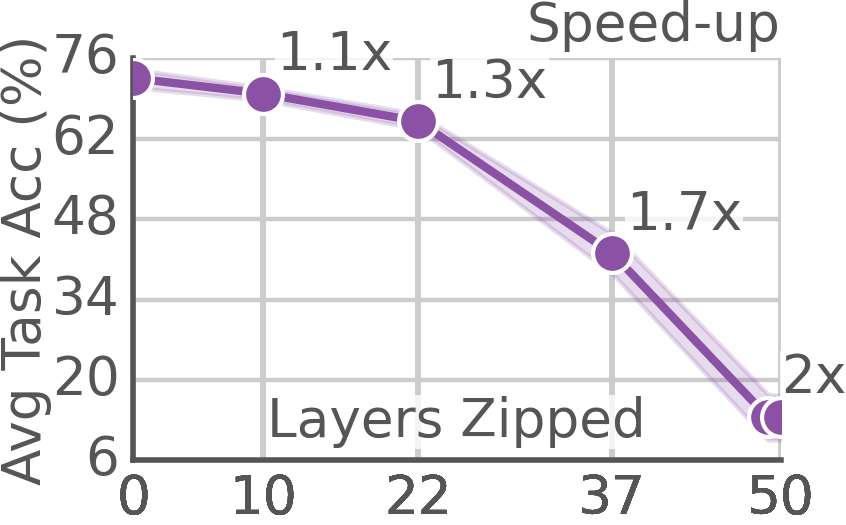
\includegraphics[width=\linewidth]{figures/imgs/partial_zip_imnet_200_200.png}
%             }\end{minipage}
%         }
%         \caption{{\bf Varying Partial Zip.} 
%             By leaving some layers unzipped (Sec.~\ref{sec:partial_zip}), we can recover a significant amount of performance while still merging most of the model.  }
%         \label{fig:varying_partial_zip}
%         % \vspace{-80pt}
%     \end{minipage}
%     \hspace{1pt}
%     % \vspace{1em} % Add vertical space between the images
%     \begin{minipage}[t]{0.48\linewidth}
%         \centering
%         \subfloat[
%             \textbf{CIFAR-100 (50+50).}
%             \label{fig:data_use_cifar100}
%         ]{
%             \centering
%             \begin{minipage}{0.48\linewidth}{
%                 \centering
%                 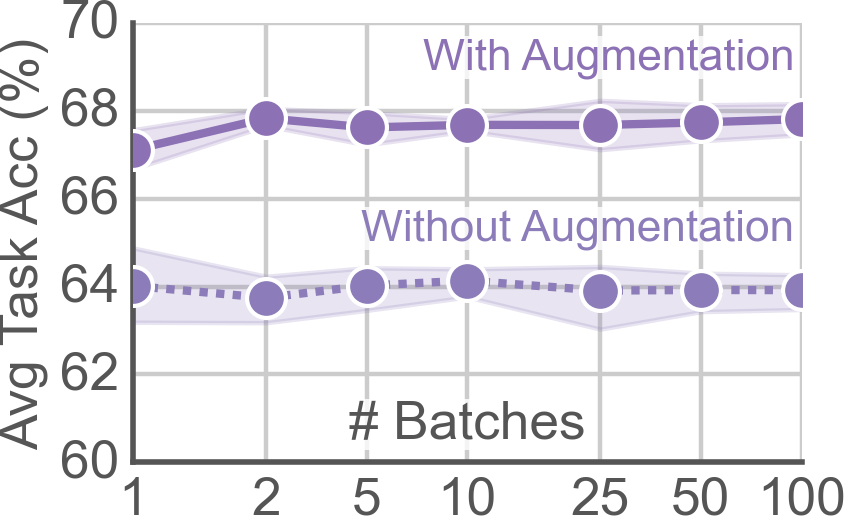
\includegraphics[width=\linewidth]{figures/imgs/cifar100_data.png}
%             }\end{minipage}
%         }
%         \subfloat[
%             \textbf{ImageNet-1k (200+200).}
%             \label{fig:data_use_imagenet}
%         ]{
%             \centering
%             \begin{minipage}{0.48\linewidth}{
%                 \centering
%                 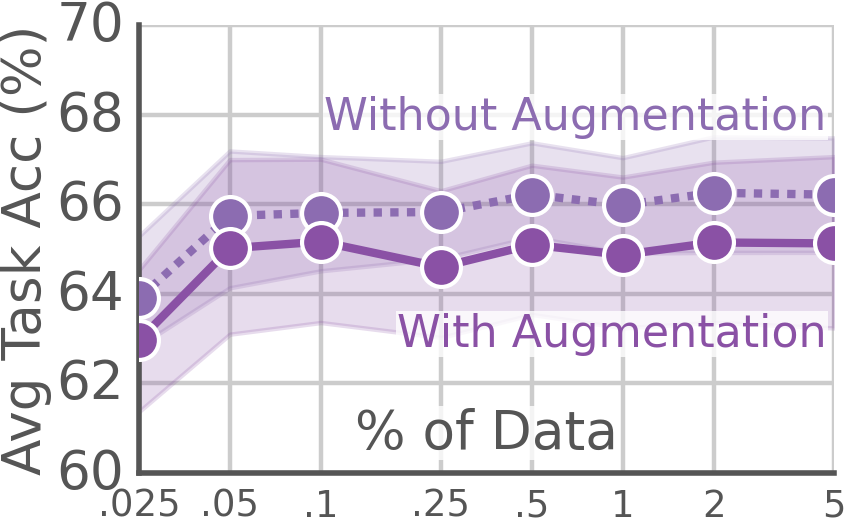
\includegraphics[width=\linewidth]{figures/imgs/imnet200_data.png}
%             }\end{minipage}
%         }
%         \caption{
%         {\bf Data Usage.} How much data do we need to use to compute activations? Here we ablate the amount of data used for our CIFAR-100 (50+50) ResNet-20 ($8\times$ width) and ImageNet (200+200) Resnet-50 (\sfrac{22}{50} layers) experiments. The batch size used is 500 for CIFAR and 16 for ImageNet. In both cases, we only need a few hundred images to obtain the best results. On the other hand, data augmentation is necessary for CIFAR but hurts for ImageNet. Our default for all experiments uses data augmentation and the full set for CIFAR (100 batches) and 1\% of the data for ImageNet. 
%         }
%         \label{fig:data_usage}
%         % \vspace{10pt}
%     \end{minipage}
%     % \caption{Overall caption for the three images}
%     \vspace{-20pt}
% \end{figure}

% \begin{wrapfigure}{r}{0.48\linewidth}
% \vspace{-10pt}
% \centering
% \resizebox{\linewidth}{!}{
%     \tablestyle{5pt}{1.1}
%     {
%     \tablestyle{5pt}{1.1}
%     \begin{tabular}{x{40}x{40}x{40}}
%         \multicolumn{3}{c}{Average Stage Correlations}\\
%         Layer \sfrac{7}{20} & Layer \sfrac{13}{20} & Layer \sfrac{19}{20}\\
%     \shline
%     {0.50\conf{0.01}} & {0.37\conf{0.00}} & {0.27\conf{0.00}} \\
%     \hline
% \end{tabular}
%     }
% }
% \captionof{table}{\textbf{CIFAR-100 (50+50) Zipping Correlations.} We show the average correlations between two ResNet-20 ($8\times$) models at each partial zipping stage. Correlations consistently decrease at each successive stage, indicating that the layers of the two models increasingly diverge. 
% }
% \label{tab:partialzip_corrs}
% % \end{table}
% \vspace{-20pt}
% \end{wrapfigure}



\section{Data Usage} \label{ap:data_usage}
In our approach, we use a sample of the training set in order to compute activations and match features together. For the main paper, we used the full training set for CIFAR, 1\% of the training set for ImageNet, and the number of images in the smallest training set for the Multi-Dataset classification experiment (so that we could use the same number of images from each dataset). In each case, we used the same data augmentations from training.

That begs the question: how much data do we actually need, and how necessary are data augmentations?
Here we ablate the amount of data used for our CIFAR-100 (50+50) ResNet-20 ($8\times$ width) and ImageNet (200+200) Resnet-50 (\sfrac{22}{50} layers) experiments. 
In Fig.~\ref{fig:data_usage}, we test how much data is actually necessary to obtain a good accuracy on CIFAR and ImageNet with or without data augmentation.

% \begin{figure}[h]
% \centering
% %
% \subfloat[
%     \textbf{CIFAR-100 (50+50).}
%     \label{fig:data_use_cifar100}
% ]{
% \centering
% \begin{minipage}{0.48\linewidth}{
% \begin{center}
%     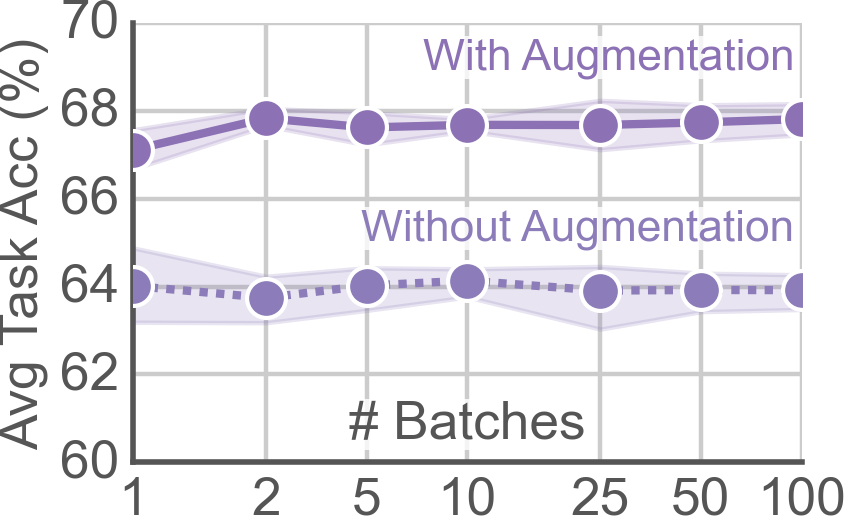
\includegraphics[width=\linewidth]{figures/imgs/cifar100_data.png}
% \end{center}
% }\end{minipage}
% }
% \subfloat[
%     \textbf{ImageNet-1k (200+200).}
%     \label{fig:data_use_imagenet}
% ]{
% \centering
% \begin{minipage}{0.48\linewidth}{
% \begin{center}
%     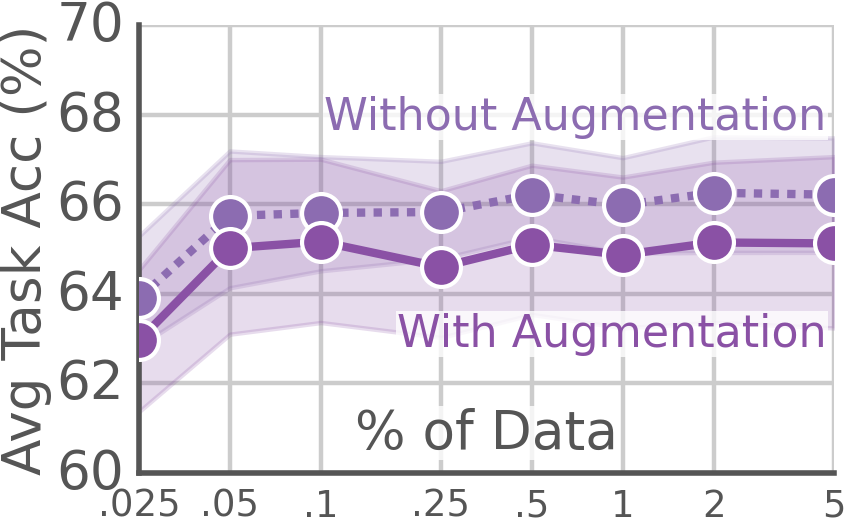
\includegraphics[width=\linewidth]{figures/imgs/imnet200_data.png}
% \end{center}
% }\end{minipage}
% }

% \caption{{\bf Data Usage.} How much data do we need to use to compute activations? Here we ablate the amount of data used for our CIFAR-100 (50+50) ResNet-20 ($8\times$ width) and ImageNet (200+200) Resnet-50 (\sfrac{22}{50} layers) experiments. The batch size used is 500 for CIFAR and 16 for ImageNet. In both cases, we only need a few hundred images to obtain the best results. On the other hand, data augmentation is necessary for CIFAR but hurts for ImageNet. Our default for all experiments uses data augmentation and the full set for CIFAR (100 batches) and 1\% of the data for ImageNet. }
% \label{fig:data_usage}
% \end{figure}



% \begin{wrapfigure}{l}{0.52\linewidth}
% % \vspace{-260pt}
% \begin{minipage}[l]{\linewidth}{
% \subfloat[
%     \textbf{CIFAR-100 (50+50).}
%     \label{fig:data_use_cifar100}
% ]{
% \centering
% \begin{minipage}{0.48\linewidth}{
% \begin{center}
%     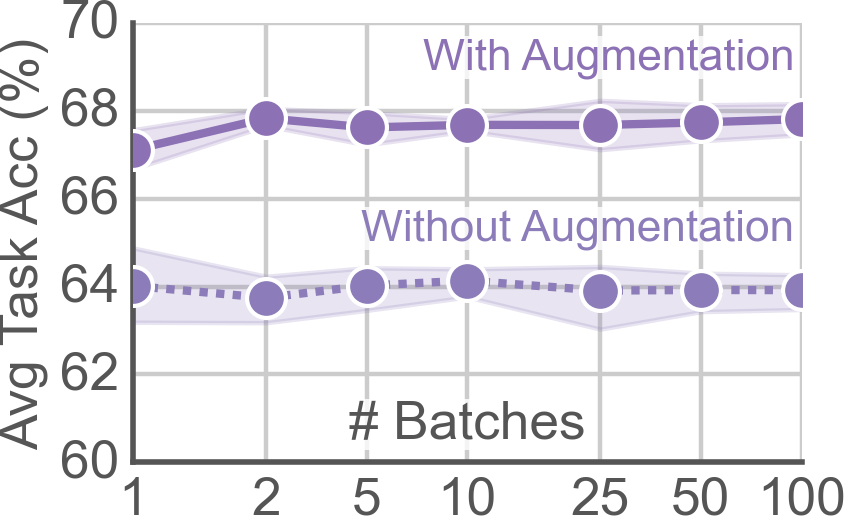
\includegraphics[width=\linewidth]{figures/imgs/cifar100_data.png}
% \end{center}
% }\end{minipage}
% }
% \subfloat[
%     \textbf{ImageNet-1k (200+200).}
%     \label{fig:data_use_imagenet}
% ]{
% \centering
% \begin{minipage}{0.48\linewidth}{
% \begin{center}
%     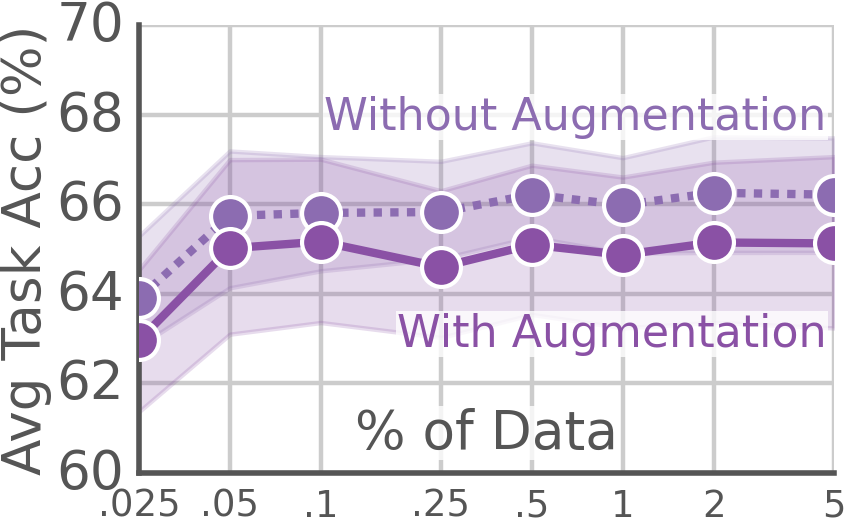
\includegraphics[width=\linewidth]{figures/imgs/imnet200_data.png}
% \end{center}
% }\end{minipage}
% }
%         \caption{
%         {\bf Data Usage.} How much data do we need to use to compute activations? Here we ablate the amount of data used for our CIFAR-100 (50+50) ResNet-20 ($8\times$ width) and ImageNet (200+200) Resnet-50 (\sfrac{22}{50} layers) experiments. The batch size used is 500 for CIFAR and 16 for ImageNet. In both cases, we only need a few hundred images to obtain the best results. On the other hand, data augmentation is necessary for CIFAR but hurts for ImageNet. Our default for all experiments uses data augmentation and the full set for CIFAR (100 batches) and 1\% of the data for ImageNet. 
%         }
% \label{fig:data_usage}
% }\end{minipage}
% \end{wrapfigure}

We ultimately find that the amount of data doesn't actually matter that much. In the main paper, we use the entire training set for CIFAR-100 with a batch size of 500 (100 batches, or 50,000 images), but it seems like as little as 2 batches (100 images) produces the same result. Similarly on ImageNet, using 0.05\% of the data (640 images) produces the same result as 5\% (64,048 images).

In fact, the main consideration is whether or not to use data augmentation. For less diverse datasets like CIFAR-100, data augmentation seems essential (giving an almost 4\% boost in average task accuracy), and well above the variance of results without augmentation. However, for ImageNet, which has much more diverse images, data augmentation actually hurts slightly on average---though the two are within variance. Note that despite this result, for consistency we use data augmentation in \textit{all} experiments.


\section{Zip Propagation Details} \label{ap:prop_rules}
In the main paper we described general rules for zip propagation---namely, propagate through layers until you reach a module with a weight matrix. Here, we describe rules more concretely for each layer type needed to define most convnets.

\paragraph{Linear.} Apply \modelc{$M_i$} and \modelc{$U_i$}. Stop propagation.

\paragraph{Conv.} Apply \modelc{$M_i$} and \modelc{$U_i$} to each kernel location (i.e., move the $k\times k$ kernel dimensions to the batch dimension). Stop propagation.

\paragraph{BatchNorm.} Apply \modelc{$M_i$} to all parameters (weight, bias, mean, variance), squaring it for the variance term. Continue propagation. As \citet{jordan2022repair} points out, we cannot compute the correct variance without knowing the covariance between the two models (which we don't have access to). Thus, we reset batch norms after merging to evaluate the variance correctly. 

\paragraph{LayerNorm.} Apply \modelc{$M_i$} to all parameters (weight, bias). Continue propagation. Since LayerNorm computes mean and standard deviation on the fly, we don't need to do anything special.

\paragraph{ReLU.} Nothing to merge. Continue propagation. Note that passing the merge matrix unchanged through the ReLU layers is an approximation, since we're using a linear merge operation on nonlinear features. Addressing this issue could be an interesting topic for future work, as even the permute and add approach of prior work has this issue (ReLU is invariant to permutation, but certainly not adding). 

\paragraph{Avg / Max Pool.} Nothing to Merge. Continue propagation.

\paragraph{Skip Connection.} Continue propagation through every input to the skip connection (using the same \modelc{$M_i$} and \modelc{$U_i$} for each).


\section{Cross Entropy on CIFAR}
% %##################################################################################################
% \begin{wrapfigure}{r}{0.48\linewidth}
% % \vspace{-10pt}
% % \begin{table}[t]
% \resizebox{\linewidth}{!}{
%     \tablestyle{5pt}{1.1}
%     {\renewcommand\conf[1]{}
%     \tablestyle{5pt}{1.1}
% \centering
% \begin{center}
% \tablestyle{5pt}{1.1}
% \begin{tabular}{y{56}x{40}|x{30}x{30}x{30}x{30}}
%         & & \multicolumn{4}{c}{Accuracies (\%)}\\
%         Method & FLOPs (G) & Joint & \modela{Task A} & \modelb{Task B} & Avg \\
%     \shline
%     \modela{Model A}                        & {10.88} & {37.9\conf{0.2}} & {74.15\conf{0.6}} & {1.7\conf{0.3}} & {36.4\conf{0.7}} \\
%     \modelb{Model B}                        & {10.88} & {36.7\conf{1.2}} & {2.2\conf{0.5}} & {75.2\conf{2.3}} & {38.7\conf{1.1}} \\
%     \hline
%     W. Avg                                  &  10.88     & {2.7\conf{0.1}}           & {5.0\conf{3.3}}           & {4.9\conf{1.2}}           & {4.9\conf{0.1}} \\
%     Git Re-Basin$\ddag$                     &  10.88     & {3.1\conf{0.8}}           & {5.8\conf{0.9}}           & {5.3\conf{0.8}}           & {5.6\conf{0.8}}  \\
%     Permute                                 &  10.88     & {20.0\conf{1.3}}          & {30.8\conf{3.3}}          & {32.8\conf{1.6}}          & {31.8\conf{1.7}} \\
%     \default{{\bf \name{}}$_\text{20/20}$}  &  10.88     & \textbf{27.9\conf{1.5}}   & \textbf{40.1\conf{2.4}}   & \textbf{39.7\conf{1.6}}   & \textbf{39.9\conf{1.9}} \\
%     \hline
%     \gc{Ensemble}                           & \gc{21.76} & \gc{60.5\conf{1.0}}       & \gc{74.2\conf{0.6}}       & \gc{75.2\conf{2.3}}       &  \gc{74.7\conf{1.4}} \\
%     \default{{\bf \name{}}$_\text{13/20}$}  & {14.52}    & {38.6\conf{2.4}}          & {51.8\conf{1.6}}          & {52.0\conf{3.5}}          & {51.9\conf{2.4}} \\
%     \default{{\bf \name{}}$_\text{7/20}$}   & {18.14}    &  \textbf{47.0\conf{2.2}}         &  \textbf{60.6\conf{1.2}}         & \textbf{60.5\conf{3.2}}          & \textbf{60.6\conf{2.1}} \\
% \end{tabular}
% \end{center}
% % \end{table}
% }
% }
% \caption{\textbf{CIFAR-100 (50+50) with Cross Entropy.} \name{}\ vs. baselines using ResNet-20 ($16\times$ width). Merging the entire model as in prior work produces bad results when using cross-entropy, hence we use CLIP in the main draft. If we use partial zipping, we can recover a lot of the lost performance. $\ddag$ refers to \cite{ainsworth2022git}
% }
% % \vspace{-20pt}
% \label{tab:cifar_ce_results}
% \end{wrapfigure}

\begin{wrapfigure}{r}{0.48\linewidth}
\vspace{-10pt}
\centering
\resizebox{\linewidth}{!}{
    \tablestyle{5pt}{1.1}
    {\renewcommand\conf[1]{}
    \tablestyle{5pt}{1.1}
    \begin{tabular}{y{56}x{40}|x{30}x{30}x{30}x{30}}
        & & \multicolumn{4}{c}{Accuracies (\%)}\\
        Method & FLOPs (G) & Joint & \modela{Task A} & \modelb{Task B} & Avg \\
    \shline
    \modela{Model A}                        & {10.88} & {37.9\conf{0.2}} & {74.15\conf{0.6}} & {1.7\conf{0.3}} & {36.4\conf{0.7}} \\
    \modelb{Model B}                        & {10.88} & {36.7\conf{1.2}} & {2.2\conf{0.5}} & {75.2\conf{2.3}} & {38.7\conf{1.1}} \\
    \hline
    W. Avg                                  &  10.88     & {2.7\conf{0.1}}           & {5.0\conf{3.3}}           & {4.9\conf{1.2}}           & {4.9\conf{0.1}} \\
    Git Re-Basin$\ddag$                     &  10.88     & {3.1\conf{0.8}}           & {5.8\conf{0.9}}           & {5.3\conf{0.8}}           & {5.6\conf{0.8}}  \\
    Permute                                 &  10.88     & {20.0\conf{1.3}}          & {30.8\conf{3.3}}          & {32.8\conf{1.6}}          & {31.8\conf{1.7}} \\
    \default{{\bf \name{}}$_\text{20/20}$}  &  10.88     & \textbf{27.9\conf{1.5}}   & \textbf{40.1\conf{2.4}}   & \textbf{39.7\conf{1.6}}   & \textbf{39.9\conf{1.9}} \\
    \hline
    \gc{Ensemble}                           & \gc{21.76} & \gc{60.5\conf{1.0}}       & \gc{74.2\conf{0.6}}       & \gc{75.2\conf{2.3}}       &  \gc{74.7\conf{1.4}} \\
    \default{{\bf \name{}}$_\text{13/20}$}  & {14.52}    & {38.6\conf{2.4}}          & {51.8\conf{1.6}}          & {52.0\conf{3.5}}          & {51.9\conf{2.4}} \\
    \default{{\bf \name{}}$_\text{7/20}$}   & {18.14}    &  \textbf{47.0\conf{2.2}}         &  \textbf{60.6\conf{1.2}}         & \textbf{60.5\conf{3.2}}          & \textbf{60.6\conf{2.1}} \\
\end{tabular}
    }
}
\captionof{table}{\textbf{CIFAR-100 (50+50) Cross Entropy.} \name{}\ vs. baselines using ResNet-20 ($16\times$ width). Merging the entire model as in prior work produces bad results when using cross-entropy, hence we use CLIP in the main draft. If we use partial zipping, we can recover a lot of the lost performance. $\ddag$ refers to \cite{ainsworth2022git}
% all pairs (2-way merging) and per-task accuracy for each head (4-way merging).
% We compare to our strong baseline as \cite{ainsworth2022git} doesn't support models with different outputs.
}
\label{tab:cifar_ce_results}
% \end{table}
\vspace{-20pt}
\end{wrapfigure}

% different run 
% \begin{center}
% \tablestyle{5pt}{1.1}
% \begin{tabular}{y{56}x{20}x{28}|x{24}x{24}x{24}}
%     & FLOPs& Joint & \multicolumn{3}{c}{Per-Task (\%)}\\
%     Method & (G) & Acc (\%) & \modela{Task A} & \modelb{Task B} & Avg\\
%     \shline
%     \modela{Model A}                        & {10.88} & {33.3\conf{0.7}} & {36.3\conf{0.4}} & {70.6\conf{1.3}} & {2.03\conf{0.7}} \\
%     \modelb{Model B}                        & {10.88} & {35.8\conf{1.1}} & {36.8\conf{1.1}} & {1.9\conf{0.5}} & {71.7\conf{2.3}} \\
%     \hline
%     W. Avg                                  &  10.88     & {6.7\conf{0.7}}           & {9.5\conf{0.7}}           & {0.1\conf{4.6}}           & {11.0\conf{5.4}} \\
%     Git Re-Basin \cite{ainsworth2022git}    &  10.88     & {1.0\conf{0.0}}           & {2.1\conf{0.1}}           & {2.0\conf{0.1}}           & {2.1\conf{0.1}}  \\
%     Permute                                 &  10.88     & {31.5\conf{3/3}}          & {46.0\conf{3.7}}          & {45.9\conf{3.2}}          & {46.0\conf{6.5}} \\
%     \default{{\bf \name{}}$_\text{20/20}$}  &  10.88     & \textbf{38.2\conf{1.5}}   & \textbf{52.5\conf{2.0}}   & \textbf{52.0\conf{2.9}}   & \textbf{52.9\conf{4.0}} \\
%     \hline
%     \gc{Ensemble}                           & \gc{21.76} & \gc{54.8\conf{1.1}}       & \gc{71.2\conf{1.2}}       & \gc{70.6\conf{1.3}}       &  \gc{71.7\conf{2.3}} \\
%     \default{{\bf \name{}}$_\text{13/20}$}  & {14.52}    & {51.2\conf{1.1}}          & {67.4\conf{1.2}}          & {66.7\conf{2.0}}          & {68.2\conf{1.9}} \\
%     \default{{\bf \name{}}$_\text{7/20}$}   & {18.14}    &  \textbf{51.6\conf{0.4}}         &  \textbf{67.5\conf{0.8}}         & \textbf{66.9\conf{2.3}}          & \textbf{68.0\conf{1.4}} \\
% \end{tabular}
% \end{center}
% % }\end{minipage}
% % }

% \caption{\textbf{CIFAR-100 (50+50) with Cross Entropy.} \name{}\ vs. baselines using ResNet-20 ($16\times$ width). Merging the entire model as in prior work produces bad results when using cross-entropy, hence we use CLIP in the main draft. If we use partial zipping, we can recover a lot of the lost performance.
% }
% \label{tab:cifar_results}
% \end{table}




% \begin{table}[t]
% \centering
% \tablestyle{5pt}{1.1}
% \begin{tabular}{y{56}x{20}x{28}|x{24}x{24}x{24}}
%     & FLOPs& Joint & \multicolumn{3}{c}{Per-Task (\%)}\\
%     Method & (G) & Acc (\%) & \modela{Task A} & \modelb{Task B} & Avg\\
%     \shline
%     \modela{Model A} & {2.72} & {33.0\conf{1.2}} & {68.1\conf{0.5}} & {1.7\conf{0.3}} & {34.9\conf{0.2}} \\
%     \modelb{Model B} & {2.72} & {35.6\conf{0.5}} & {1.7\conf{0.4}} & {71.6\conf{0.8}} & {36.7\conf{0.5}} \\
%     \hline
%     W. Avg \tiny{(Eq.~\ref{eq:wavg})} &2.72& {1.3\conf{.1}} & {2.8\conf{0.5}} & {2.6\conf{0.3}} & {2.7\conf{0.2}} \\
%     Git Re-Basin \cite{ainsworth2022git}  &2.72 & {1.7\conf{0.4}} & {2.9\conf{0.5}} & {3.5\conf{0.5}} & {3.2\conf{0.5}}  \\
%     Permute \tiny{(Eq.~\ref{eq:rebasin})} &2.72 & \textbf{9.2\conf{0.9}} & \textbf{14.9\conf{0.6}} & \textbf{17.2\conf{1.9}} & \textbf{16.1\conf{1.2}} \\
%     \default{{\bf \name{}}$_\text{20/20}$} &2.72 & \textbf{8.4\conf{0.9}} & \textbf{14.5\conf{1.7}} & \textbf{15\conf{1.2}} & \textbf{14.8\conf{1.4}} \\
%     \hline
%     \gc{Ensemble} & \gc{5.45} & \gc{55.7\conf{1.5}} & \gc{68.1\conf{2.3}} & \gc{71.6\conf{0.8}} & \gc{69.8\conf{1.5}} \\
%     \default{{\bf \name{}}$_\text{13/20}$} & 3.63 & {25.0\conf{2.0}} & {24.5\conf{0.8}} & {26.8\conf{2.2}} & {25.6\conf{1.3}} \\
% \end{tabular}

% \caption{\textbf{CIFAR50+50 ResNet20x8 Results.}
% }
% \label{tab:r20x8_c50logits}
% \end{table}
% %##################################################################################################
In the main paper, we train our CIFAR models with a CLIP \cite{radford2021learning} loss (using CLIP embeddings of class names as targets). This ensures that the output spaces of the two models are aligned, which is necessary to get good accuracy for prior work that merge the entire model together. 

\paragraph{ResNet.} In Tab.~\ref{tab:cifar_ce_results}, we show results for CIFAR-100 (50+50) where we train with the normal one-hot targets (i.e., like we did for ImageNet), instead. Immediately, we see that accuracies of the merged models are much lower across the board, with no method able to outperform just using one of the original models when merging the entire network. In fact, Git Re-Basin \cite{ainsworth2022git} does almost no better than weight averaging, which gets close to random accuracy. While \name{}\ without partial zipping also performs worse than the original models, it still greatly outperforms all prior work. And with partial zipping, \name{}\ is able to exceed the accuracy of the original models.

Thus, in the case of using cross-entropy loss, partial zipping is extremely important. Merging the entire model as in prior work fails, since the later layers of the model are incompatible with each other due to each model having a different output space. Partial zipping, on the other hand, can mitigate that issue.


% %##################################################################################################
% \begin{table}[t]
% \centering
% \begin{center}
% \tablestyle{5pt}{1.1}
% \begin{tabular}{y{56}x{20}x{28}|x{24}x{24}x{24}}
%     & FLOPs& Joint & \multicolumn{3}{c}{Per-Task (\%)}\\
%     Method & (G) & Acc (\%) & \modela{Task A} & \modelb{Task B} & Avg\\
%     \shline
%     \modela{Model A}                        & {0.15} & {44.6\conf{1.0}} & {89.2\conf{2.0}} & {21.0\conf{1.5}} & {55.1\conf{1.5}} \\
%     \modelb{Model B}                        & {0.15} & {44.0\conf{1.4}} & {23.1\conf{4.5}} & {88.1\conf{2.8}} & {55.6\conf{3.4}} \\
%     \hline
%     W. Avg                                  &  0.15     & {10.2\conf{0.2}}           & {20.8\conf{1.2}}           & {20.9\conf{0.7}}           & {20.9\conf{0.7}} \\
%     Permute                                 &  0.15     & {25.4\conf{1.1}}          & {47.2\conf{1.3}}          & {48.5\conf{12.3}}          & {47.8\conf{5.8}} \\
%     \default{{\bf \name{}}$_\text{22/22}$}  &  0.15     & \textbf{33.2\conf{9.3}}   & \textbf{53.8\conf{14.7}}   & \textbf{59.9\conf{9.6}}   & \textbf{56.5\conf{6.5}} \\
%     \hline
%     \gc{Ensemble}                           & \gc{0.30} & \gc{66.6\conf{2.5}}       & \gc{89.2\conf{2.0}}       & \gc{88.1\conf{2.8}}       &  \gc{88.6\conf{0.5}} \\
%     \default{{\bf \name{}}$_\text{14/22}$}  & {0.17}    & {35.2\conf{6.0}}          & {56.7\conf{13.7}}          & {60.2\conf{15.9}}          & {58.4\conf{5.9}} \\
%     \default{{\bf \name{}}$_\text{7/22}$}   & {0.27}    &  \textbf{44.5\conf{2.9}}  &  \textbf{66.0\conf{4.2}}    & \textbf{65.1\conf{11.2}} & \textbf{65.5\conf{4.1}} \\
% \end{tabular}
% \end{center}
% % }\end{minipage}
% % }

% \caption{\textbf{CIFAR-10 (5+5) CE with VGG.} \name{}\ vs. baselines using VGG11 ($1\times$ width) using Cross Entropy instead of CLIP loss. \name{} displays the same behavior here as it does for ResNet-20 with low width. Note that this is CIFAR-10 not CIFAR-100.
% }
% \label{tab:cifar5_vgg11w1_results}
% \end{table}


\begin{wrapfigure}{r}{0.48\linewidth}
\vspace{-10pt}
\centering
\resizebox{\linewidth}{!}{
    \tablestyle{5pt}{1.1}
    {\renewcommand\conf[1]{}
    \tablestyle{5pt}{1.1}
    \begin{tabular}{y{56}x{40}|x{30}x{30}x{30}x{30}}
        & & \multicolumn{4}{c}{Accuracies (\%)}\\
        Method & FLOPs (G) & Joint & \modela{Task A} & \modelb{Task B} & Avg \\
    \shline
    \modela{Model A}                        & {0.15} & {44.6\conf{1.0}} & {89.2\conf{2.0}} & {21.0\conf{1.5}} & {55.1\conf{1.5}} \\
    \modelb{Model B}                        & {0.15} & {44.0\conf{1.4}} & {23.1\conf{4.5}} & {88.1\conf{2.8}} & {55.6\conf{3.4}} \\
    \hline
    W. Avg                                  &  0.15     & {10.2\conf{0.2}}           & {20.8\conf{1.2}}           & {20.9\conf{0.7}}           & {20.9\conf{0.7}} \\
    Permute                                 &  0.15     & {25.4\conf{1.1}}          & {47.2\conf{1.3}}          & {48.5\conf{12.3}}          & {47.8\conf{5.8}} \\
    \default{{\bf \name{}}$_\text{22/22}$}  &  0.15     & \textbf{33.2\conf{9.3}}   & \textbf{53.8\conf{14.7}}   & \textbf{59.9\conf{9.6}}   & \textbf{56.5\conf{6.5}} \\
    \hline
    \gc{Ensemble}                           & \gc{0.30} & \gc{66.6\conf{2.5}}       & \gc{89.2\conf{2.0}}       & \gc{88.1\conf{2.8}}       &  \gc{88.6\conf{0.5}} \\
    \default{{\bf \name{}}$_\text{14/22}$}  & {0.17}    & {35.2\conf{6.0}}          & {56.7\conf{13.7}}          & {60.2\conf{15.9}}          & {58.4\conf{5.9}} \\
    \default{{\bf \name{}}$_\text{7/22}$}   & {0.27}    &  \textbf{44.5\conf{2.9}}  &  \textbf{66.0\conf{4.2}}    & \textbf{65.1\conf{11.2}} & \textbf{65.5\conf{4.1}} \\
\end{tabular}
    }
}
\captionof{table}{\textbf{CIFAR-10 (5+5) CE with VGG.} \name{}\ vs. baselines using VGG11 ($1\times$ width) using Cross Entropy instead of CLIP loss. \name{} displays the same behavior here as it does for ResNet-20 with low width. 
% Note that this is CIFAR-10 not CIFAR-100.
% all pairs (2-way merging) and per-task accuracy for each head (4-way merging).
% We compare to our strong baseline as \cite{ainsworth2022git} doesn't support models with different outputs.
}
\label{tab:cifar5_vgg11w1_results}
% \end{table}
\vspace{-10pt}
\end{wrapfigure}

\paragraph{VGG.}\label{ap:vgg}
In the main paper, we use ResNets for each experiment, since they are easy to train and produce strong results. However, in principle \name{}\ can work on any architecture. For completeness, in Tab.~\ref{tab:cifar5_vgg11w1_results}, we show results on the CIFAR-10 (5+5) setting with VGG11 ($1\times$ width). Note that this is a much smaller and weaker model than the ResNet-20s we use in the main paper, so its results on CIFAR-10 aren't as strong. Furthermore, we conducted this experiment with a cross entropy loss, so merging the entire model performs worse than the original models.

Despite this, we observe a very similar trend to the ResNet-20 models in that \name{}\ outperforms all baselines and that partial zipping is important for reaching the accuracy of the original models (in this case, matching not exceeding). In fact, these results continue a more general trend in that \name{}\ greatly benefits from larger model scales, making effective use of the extra capacity. In this case, the scale of the model is quite small, so there is not as much room in the weights to store the potentially disjoint features of both models.


% \begin{table}[t]
% \centering
% \tablestyle{5pt}{1.1}
% \begin{tabular}{y{56}x{20}x{28}|x{24}x{24}x{24}}
%     & FLOPs& Joint & \multicolumn{3}{c}{Per-Task (\%)}\\
%     Method & (G) & Acc (\%) & \modela{Task A} & \modelb{Task B} & Avg\\
%     \shline
%     \multicolumn{6}{c}{$1\times$ Width} \\
%     \hline
%     \gc{Ensemble} & \gc{8.22} & \gc{63.3\conf{4.9}} & \gc{74.3\conf{4.0}} & \gc{70.5\conf{3.2}} & \gc{72.4\conf{2.5}} \\
%     \default{{\bf \name{}}$_\text{50/50}$} & 4.11 & {8.6\conf{4.7}} & {12.4\conf{5.9}} & {14.7\conf{7.8}} & {13.5\conf{6.6}} \\
%     \default{{\bf \name{}}$_\text{37/50}$} & 4.92 & {33.1\conf{5.9}} & {41.8\conf{5.3}} & {42.3\conf{8.2}} & {42.0\conf{6.2}} \\
%     \default{{\bf \name{}}$_\text{22/50}$} & 6.39 & {55.8\conf{4.1}} & {65.9\conf{2.5}} & {64.1\conf{3.0}} & {65.0\conf{2.3}} \\
%     \default{{\bf \name{}}$_\text{10/50}$} & 7.43 & {60.9\conf{4.1}} & {70.7\conf{3.0}} & {69.0\conf{2.9}} & {69.9\conf{1.9}} \\
%     \hline
%     \multicolumn{6}{c}{$1.5\times$ Width} \\
%     \hline
%     \gc{Ensemble} & \gc{32.6} & \gc{67.8\conf{3.5}} & \gc{76.7\conf{4.1}} & \gc{72.6\conf{2.8}} & \gc{74.7\conf{2.5}} \\
%     \default{{\bf \name{}}$_\text{50/50}$} & 16.3 & {9.7\conf{6.9}} & {13.2\conf{9.5}} & {16.0\conf{10.0}} & {14.6\conf{9.3}} \\
%     \default{{\bf \name{}}$_\text{37/50}$} & 19.5 & {49.0\conf{2.5}} & {56.2\conf{4.2}} & {56.7\conf{2.1}} & {56.4\conf{2.8}} \\
%     \default{{\bf \name{}}$_\text{22/50}$} & 25.5 & {64.1\conf{2.7}} & {71.6\conf{2.3}} & {70.4\conf{2.3}} & {71.0\conf{1.8}} \\
%     \default{{\bf \name{}}$_\text{10/50}$} & 29.7 & {66.8\conf{3.2}} & {74.9\conf{3.5}} & {72.1\conf{2.3}} & {73.5\conf{2.1}} \\
% \end{tabular}

% \caption{\textbf{ImageNet-1k (200+200) Width Comparison.} We show how \name{}\ is able to make use of the extra model width when merging models together. For instance, merging 37 layers goes from 33\% joint accuracy with $1\times$ width to 49\% with $1.5\times$, while the ensemble only improves by 4\%. Because these models use cross-entropy, merging the entire network still results in poor performance.
% }
% \label{tab:imagenet200x5width}
% \end{table}

\begin{wrapfigure}{r}{0.48\linewidth}
\vspace{-10pt}
\centering
\resizebox{\linewidth}{!}{
    \tablestyle{5pt}{1.1}
    {\renewcommand\conf[1]{}
    \tablestyle{5pt}{1.1}
    \begin{tabular}{y{56}x{40}|x{30}x{30}x{30}x{30}}
        & & \multicolumn{4}{c}{Accuracies (\%)}\\
        Method & FLOPs (G) & Joint & \modela{Task A} & \modelb{Task B} & Avg \\
    \shline
    \multicolumn{6}{c}{$1\times$ Width} \\
    \hline
    \gc{Ensemble} & \gc{8.22} & \gc{63.3\conf{4.9}} & \gc{74.3\conf{4.0}} & \gc{70.5\conf{3.2}} & \gc{72.4\conf{2.5}} \\
    \default{{\bf \name{}}$_\text{50/50}$} & 4.11 & {8.6\conf{4.7}} & {12.4\conf{5.9}} & {14.7\conf{7.8}} & {13.5\conf{6.6}} \\
    \default{{\bf \name{}}$_\text{37/50}$} & 4.92 & {33.1\conf{5.9}} & {41.8\conf{5.3}} & {42.3\conf{8.2}} & {42.0\conf{6.2}} \\
    \default{{\bf \name{}}$_\text{22/50}$} & 6.39 & {55.8\conf{4.1}} & {65.9\conf{2.5}} & {64.1\conf{3.0}} & {65.0\conf{2.3}} \\
    \default{{\bf \name{}}$_\text{10/50}$} & 7.43 & {60.9\conf{4.1}} & {70.7\conf{3.0}} & {69.0\conf{2.9}} & {69.9\conf{1.9}} \\
    \hline
    \multicolumn{6}{c}{$1.5\times$ Width} \\
    \hline
    \gc{Ensemble} & \gc{32.6} & \gc{67.8\conf{3.5}} & \gc{76.7\conf{4.1}} & \gc{72.6\conf{2.8}} & \gc{74.7\conf{2.5}} \\
    \default{{\bf \name{}}$_\text{50/50}$} & 16.3 & {9.7\conf{6.9}} & {13.2\conf{9.5}} & {16.0\conf{10.0}} & {14.6\conf{9.3}} \\
    \default{{\bf \name{}}$_\text{37/50}$} & 19.5 & {49.0\conf{2.5}} & {56.2\conf{4.2}} & {56.7\conf{2.1}} & {56.4\conf{2.8}} \\
    \default{{\bf \name{}}$_\text{22/50}$} & 25.5 & {64.1\conf{2.7}} & {71.6\conf{2.3}} & {70.4\conf{2.3}} & {71.0\conf{1.8}} \\
    \default{{\bf \name{}}$_\text{10/50}$} & 29.7 & {66.8\conf{3.2}} & {74.9\conf{3.5}} & {72.1\conf{2.3}} & {73.5\conf{2.1}} \\
\end{tabular}
    }
}
\captionof{table}{\textbf{ImageNet-1k (200+200) Width Comparison.} We show how \name{}\ is able to make use of the extra model width when merging models together. For instance, merging 37 layers goes from 33\% joint accuracy with $1\times$ width to 49\% with $1.5\times$, while the ensemble only improves by 4\%. These models use cross-entropy, so merging the entire network results in poor performance.
% all pairs (2-way merging) and per-task accuracy for each head (4-way merging).
% We compare to our strong baseline as \cite{ainsworth2022git} doesn't support models with different outputs.
}
\label{tab:imagenet200x5width}
% \end{table}
\vspace{-20pt}
\end{wrapfigure}

\section{ImageNet with 1.5x Width}
In the main paper, we show that \name{}\ scales very well with increased width of the model for the CIFAR-100 (50+50) setting. While CIFAR-100 is a challenging dataset on its own, the natural question is if that same trend occurs the much harder ImageNet-1k (200+200) setting.

In Tab.~\ref{tab:imagenet200x5width}, we test this by comparing \name{}\ on the original $1\times$ width ResNet-50 in the main paper with a $1.5\times$ width one.
In all cases, except for the fully zipped model (likely because of the Cross-Entropy loss), \name{}\ enjoys a large jump in performance from the extra width. For 37 layers, 33.1\% joint accuracy becomes 49.0\%. For 22 layers, 55.8\% becomes 64.1\%. And for 10 layers, 60.9\% becomes 66.8\%, now only 1\% away from the ensemble. Thus, even in this much more challenging setting, \name{}\ is able to make full use of the extra model capacity.

\section{Merging models with different output modalities} \label{appendix:semantic_segmentation}
\begin{wrapfigure}{r}{0.48\linewidth}
\vspace{-10pt}
\centering
\resizebox{\linewidth}{!}{
    \tablestyle{5pt}{1.1}
    {\renewcommand\conf[1]{}
    \tablestyle{5pt}{1.1}
    \begin{tabular}{y{40}|x{50}x{50}} 
                                                &      {Accuracy (\%)}      &         {mIoU (\%)}       \\
        Method                                  & \modela{ImageNet-1k}      & \modelb{Pascal VOC}       \\ 
    \shline
    W. Avg                                      & {0.8}         & {3.3}         \\
    \default{{\bf \name{}}$_\text{49/50}$}      & \textbf{23.1}            & \textbf{6.0}  \\
    \hline
    \gc{Ensemble}                               & \gc{77.8}                & \gc{76.8}                \\
    \default{{\bf \name{}}$_\text{37/50}$}      & {47.7}                   & {35.0}                   \\
    \default{{\bf \name{}}$_\text{22/50}$}      & {60.9}                   & {64.4}                   \\
    \default{{\bf \name{}}$_\text{10/50}$}      &    \textbf{64.9}         & \textbf{71.7}            \\
\end{tabular}
    }
}
\captionof{table}{\textbf{PASCAL VOC and ImageNet-1k} merging models with different output modalities using a DeepLabV3 ResNet-50 backbone and ImageNet-1k Resnet-50 model.  
}
\label{tab:voc_imagenet_results}
% \end{table}
\vspace{-10pt}
\end{wrapfigure}
In this experiment we use \name{}\ to merge two models with different initializations trained on different tasks with \textit{different} output modalities: semantic segmentation and image classification. 
Specifically, we merge the ResNet-50 backbone of a DeepLabV3 \citep{chen2017deeplabv3} model finetuned on the Pascal VOC \citep{Everingham10pascalvoc} dataset, with a ResNet-50 model trained on ImageNet-1k.
While the DeepLabV3 backbone was itself pre-trained on ImageNet-1k, it was further finetuned on Pascal VOC and does not share the initialization of our classification model. Table~\ref{tab:voc_imagenet_results} shows the results of combining the two ResNet-50 models with \name{}\ at various partial merging locations. 
% We conduct a hyperparameter search over a held-out validation set sampled from each task's validation data to find the optimal $\alpha\text{, and }\beta$ for \name{}\ at each merge location. 
We evaluate the performance of each merged by reporting its ImageNet-1k accuracy, and its Pascal VOC mIoU as is standard. 
Overall, we observe that \name{}\ is capable of merging nearly half the number of ResNet-50 layers between both models while still maintaining good performance on \textit{both tasks}, all \textit{without any training}.



% Useful Commands
\newcommand{\vv}{{\mathbf{v}}}
\newcommand{\vvP}{{\mathbf{v'}}}
\newcommand{\vvPP}{{\mathbf{v''}}}
\newcommand{\vW}{{\mathbf{W}}}
\newcommand{\vWP}{{\mathbf{W'}}}
\newcommand{\vWPP}{{\mathbf{W''}}}
\newcommand{\thetar}{\bm{\theta}_r}
\newcommand{\thetah}{\bm{\theta}_h}
% Reduced Commands
\newcommand{\vvR}{{H_{m\rightarrow r}^v(\mathbf{v})}}
\DeclarePairedDelimiter{\norm}{\lVert}{\rVert} % define a "\norm" macro

\section{A Tighter Bound for Linear Mode Connectivity}\label{ap:Theorem}
In this section we demonstrate that merging models by supporting feature merges both \textit{across} and \textit{within} each, yields a tighter bound than Theorem 3.1 in \citep{entezari2021role} in its limited setting.
We first introduce necessary background from prior work, including Theorem 3.1 and a particular formalization for within-model merging borrowed from~\citep{simsek2021geometry}.
Second, we introduce Theorem 1, which produces a tighter bound on Theorem 3.1 when merging within models is allowed, and prove its validity (Section~\ref{ap:TheoremDef} \&~\ref{ap:Theorem_proof}). 
Third, we provably extend Theorem 1 to a less restrictive setting, retaining its bounds (Section~\ref{ap:theorem1_extended}).

\subsection{Background}\label{ap:Theorem_background}
We first introduce Theorem 3.1 from \citep{entezari2021role}. Second, we formalize a restricted version of within-model merging necessary for our proof using the definitions from~\cite{simsek2021geometry}. 

\subsubsection{Thoerem 3.1}\label{ap:theorem3.1}
\paragraph{The Theorem. } Let $f_{\{\vv,\vW\}}(x)=\vv^T\sigma(\vW x)$, $f_{\{\vvP,\vWP\}}(x)=\vv'^T\sigma(\vW' x)$ be two fully-connected networks with $h$ hidden units where $\sigma(\cdot)$ is ReLU activation, $\vv\in\mathbb{R}^h$ and $\vW\in\mathbb{R}^{h\times d}$ are the parameters and $x\in\mathbb{R}^d$ is the input. If each element of $\vW$ and $\vWP$ is sampled uniformly from $[-1/\sqrt{d},1/\sqrt{d}]$ and each element of $\vv$ and $\vvP$ is sampled uniformly from $[-1/\sqrt{h},1/\sqrt{h}]$, then for any $x\in\mathbb{R}^d$ such that $\norm{x}_2=\sqrt{d}$, with probability $1-\delta$ over $\vW,\vWP, \vv, \vvP$, there exist a permutation such that

\begin{equation}
    |f_{\{\alpha\vv + (1-\alpha)\vvPP, \alpha\vW+(1-\alpha)\vWPP\}}(x) - \alpha f_{\{\vv,\vW\}}(x) - (1-\alpha)f_{\{\vvP,\vWP\}}(x)| = \Tilde{O}(h^{-\frac{1}{2d+4}})\label{eq:perm_LMC}
\end{equation}

where $\vvPP,\vWPP$ are permuted version of $\vvP,\vWP$, $\alpha\in[0,1]$ is an arbitrary interpolation constant, and the left-hand-side of the equality is the amount an interpolated model differs in output compared to the interpolation of the original models. \citep{entezari2021role} show that minimizing this quantity is analogous to minimizing the barrier (as defined by~\citet{entezari2021role}) in this setting. 
This is important because it states that achieving a zero output difference is equivalent to achieving zero-barrier, which implies that two models are linearly mode connected (LMC). 

\paragraph{Implications} Theorem 3.1 states that given any two two-layer models with different random initializations, there exists a permutation for one model such that applying the permutation makes it linearly mode connected to the second with high probability, given that the networks are \textit{wide enough} (i.e. $h$ is large enough). In other words, it states that any two randomly initialized two-layer networks are LMC modulo permutation with high likelihood. \citet{entezari2021role} use this result to conjecture that most well-trained neural networks with the same architecture and trained on the same task are also LMC modulo permutation with high likelihood. 

Notably however, permutations only allow for merging \textit{across} models. We will show how adding the ability to merge \textit{within} models leads to a tighter bound than Theorem 3.1 with the same likelihood.%, or analogously the same bound but with higher likelihood. 


% \paragraph{Preserving Function Invariance Beyond Permutations.} 
\subsubsection{A Restricted Formalization of Merging Within Models}\label{ap:reducible_def}
\paragraph{The Formalization. }
Let $\bm{\theta}_h=\{\vv,\vW\}$ represent a parameter-set such that $f_{\{\vv,\vW\}}=f_{\bm{\theta}_h}$, and likewise let $\bm{\theta'}_h=\{\vvP,\vWP\}, \text{ s.t. }, f_{\{\vvP,\vWP\}}=f_{\bm{\theta'}_h}$. 
Given $\thetah$, let $\Theta_h$ denote the set of all parameter-sets with functional equivalence to $\thetah$.
This means that $\forall \theta\in\Theta_h\text{, and }\forall x\in\{x\in\mathbb{R}^d|\  \norm{x}_2=\sqrt{d}\}, f_{\bm{\theta}}(x)=f_{\bm{\thetah}}(x)$.
Similarly, let $\Theta_h'$ be the set of all parameter-sets with functional equivalence to $\thetah'$.
Following $\bm{\theta_h}$, let $\bm{\theta}_r$ be an arbitrary parameter-set for $f$ which has $r$ hidden units instead. Assume $\bm{\theta}_h$ can be reduced to some $\bm{\theta}_r, r\leq h$ in a function-invariant manner using the definition of zero-type neurons from \citep{simsek2021geometry}. This means that there are $h-r$ total combinations of (1) rows in $\vW$ that are copies of one another whose corresponding $\vv$ elements \textit{sum to $0$}, and (2) some zero-elements in $\vv$. Thus, following \citet{simsek2021geometry} there exists a function-and-loss-preserving affine transformation that reduces $\bm{\theta}_h$ to $\bm{\theta}_r$. 
% We restrict our attention to cases where this function is linear and 
We denote this function as $M_{h\rightarrow r}\in\mathbb{R}^{r\times h}$, with $M_{h\rightarrow r}(\bm{\theta}_h)=\bm{\theta}_r$. Note that when $r=h$, $M_{h\rightarrow r}$ can simply be the identity transformation.

By definition, $\thetah$ lies in the expansion manifold of $\thetar$ \citep{simsek2021geometry}. 
This means there is a similarly defined affine transformation $U_{r\rightarrow h}\in\mathbb{R}^{h\times r}$ that can expand $\thetar$ back to arbitrary $\bm{\Tilde{\theta}_h}\in\Theta_h$ lying on the expansion manifold. 
One simple way is to extend $\thetar$ to $\bm{\Tilde{\theta}_h}$ by filling the remaining $h-r$ $\vv$ elements with $0$ and the $h-r$ $\vW$ rows with arbitrary values. 
% Under the definition, these $h-r$ neurons whose incoming weight vector copies from $\vW$ and outgoing $\vv$ elements sum to zero would be considered zero-type neurons.
Because the associated $\vv$ elements for each $\vW$ row are zero, the values of each row don't impact the function output.
% Under the definition, these $h-r$ elements would be considered zero-type neurons.
Note that because $h\geq r$, $U_{r\rightarrow h}$ can assign $\thetar$ into arbitrary new indices in $\thetah$. 
Thus, $U_{r\rightarrow h}$ act as both a \textit{permutation and expansion} transformation. 
Let $T=U\circ M=U_{r\rightarrow h}(M_{h\rightarrow r}(\thetah))$ be the coupling of the reduction and expansion affine-transformations that produce new networks of width $h$ from $\thetar$. 
By definition, any $T$ is a permutation when $M$ is the identity and $U$ is the permutation matrix. 
For the remainder of this section, we assume that $T$ further contains a permutation (i.e. $T=P\circ U\circ M$ for some permutation matrix $P\in\mathbb{R}^{h\times h}$).

We will leverage the concept of zero-type neurons presented in \citep{simsek2021geometry} to obtain a tighter bound on Theorem 3.1. 

\paragraph{A Note on Novelty.} While we borrow ideas from \citet{simsek2021geometry}, our Theorem is a differs in theoretical application. 
First, \citet{simsek2021geometry} restrict their attention to overall connectivity across points within expansion manifolds. 
% They do not explore the existence of direct-linear connectivity between two arbitrary points as in Theorem 3.1. 
This is important because our Theorem and proof do not require models to lie on the \textit{same} expansion manifold to be linearly mode connected. 
% They can instead be \textit{disconnected} over each-other's manifold. 
% Second, we seek direct-linear connectivity instead of polygonal chains. 
Second, our models need not be reducible to the same $r$. 
That is, we allow for arbitrary reducibility between any two network parameter-sets. 
% Third, our setting involves a different set of models than those studied in \citet{simsek2021geometry}. 
Our theorem also differs from Theorem 3.1 in \citep{entezari2021role} in that we extend function-invariant transformations beyond the permutation matrix, and show that tighter bounds are achievable in the process. Furthermore, we show that uniformity assumptions may be relaxed while retaining the same bounds (Section \ref{ap:theorem1_extended}).

% Let $\Omega_{r\rightarrow h}(\thetar)$ denote the expansion manifold (defined in \citep{simsek2021geometry}) of $\thetar$. For simplicity, we restrict each point in the expansion manifold to be a linear transformation of $\thetar$. We define this transformation by $U_{r\rightarrow h}\in\mathbb{R}^{h\times r}$, which expands $\thetar$ from $r$ back to width $h$. One way this can be done is 

% If $M_{h\rightarrow r}(\thetah)=\thetar$ then $\thetah$ lies in the expansion manifold of $\thetar$ as defined in \citep{simsek2021geometry}. This means that

% Under certain activations such as ReLU, we can generalize Definition 3.1 with another reducible property. More specifically, any rows in $\vW$ whose outputs are a linear combination of each other after activation can also be reduced. I.e., if there exists a set $\mathbb{S}$ of rows in $\vW$ such that $\forall x\in\mathbb{R}^d\ \exists j\notin\mathbb{S}, \sigma(\vW_j x) = \sum_{i\in \mathbb{S}} \vv_i\sigma(\vW_i x)$ where $\vv_i\in\mathbb{R}_+$ are scalar weights, then $\bm{\theta}_h$ is also reducible. 

% A second observation is that for any $M_{h\rightarrow r}\in\mathbb{R}^{r\times h}$, we can define a complementary linear transformation $U_{r\rightarrow h}\in\mathbb{R}^{h\times r}$ that expands $\bm{\theta}_r$ back to some $\bm{\theta}_h$ while preserving function and loss. One intuitive way this can be done is by copying $h-r$ arbitrary elements with appropriate normalization in $\bm{\theta}_r$ to fill $\thetah$. An even simpler way is to extend $\thetar$ to $\thetah$ by filling the remaining $h-r$ width parameters with $0$. We can do this by assigning $h-r$ elements of $\vv$ to be $0$, and then fill their corresponding $h-r$ rows of $\vW$ with any arbitrary values. Note that because $h\geq r$, $U_{r\rightarrow h}$ can assign $\thetar$ into arbitrary new indices in $\thetah$. Thus, $U_{r\rightarrow h}$ act as both a \textit{permutation and expansion} transformation. 
% Let $T=U\circ M=U_{r\rightarrow h}(M_{h\rightarrow r}(\thetah))$ be the linear coupling of the reduction and extension linear-transformations that produce new networks of width $h$ from $\thetah$. By definition, any $T$ is a permutation when $M$ is the identity and $U$ is the permutation matrix. For the remainder of this section, we assume that $T$ further contains a permutation (i.e. $T=P\circ U\circ M$ for some permutation matrix $P\in\mathbb{R}^{h\times h}$).

\subsection{A theoretical Result}\label{ap:TheoremDef}
We now introduce Theorem 1, an extension of Theoerem 3.1 that yields a strictly tighter bound when the transformations $T$ from Section~\ref{ap:reducible_def} are included and $r < h$, and exactly as tight when $r=h$. We leave the proof to the next section. 

\paragraph{Theorem 1.} 
Let $f_{\{\vv,\vW\}}(x)=\vv^T\sigma(\vW x)$, $f_{\{\vvP,\vWP\}}(x)=\vv'^T\sigma(\vW' x)$ be two fully-connected networks with $h$ hidden units where $\sigma(\cdot)$ is ReLU activation, $\vv\in\mathbb{R}^h$ and $\vW\in\mathbb{R}^{h\times d}$ are the parameters and $x\in\mathbb{R}^d$ is the input. If each element of $\vW$ and $\vWP$ is sampled uniformly from $[-1/\sqrt{d},1/\sqrt{d}]$ and each element of $\vv$ and $\vvP$ is sampled uniformly from $[-1/\sqrt{h},1/\sqrt{h}]$, then for any $x\in\mathbb{R}^d$ such that $\norm{x}_2=\sqrt{d}$, with probability $1-\delta$ over $\vW,\vWP, \vv, \vvP$, there exist transformations $T,T'$ such that
\begin{align}
    &|f_{\{\alpha\Tilde{\vv} + (1-\alpha)\Tilde{\vv}', \alpha\Tilde{\vW}+(1-\alpha)\Tilde{\vW}'\}}(x) - \alpha f_{\{\vv,\vW\}}(x) - (1-\alpha)f_{\{\vv',\vW'\}}(x)| \nonumber \\
    &\leq\begin{cases}
            \Tilde{O}\left(\left(\frac{h^2}{(r+r')-h}\right)^{-\frac{1}{2d+4}}\right) & \text{, }(r+r')-h > 0 \\
            0 &\text{, otherwise}
        \end{cases}\label{eq:T_LMC}
\end{align}
where $\Tilde{\vv},\Tilde{\vW}$ are transformed versions of $\vv,\vW$ from $T$ and $\Tilde{\vv}',\Tilde{\vW}'$ are transformed versions of $\vvP,\vWP$ from $T'$ respectively. $0 < r, r' \leq h$ are the hidden unit amounts each network can be reduced to via its respective $M,M'$ transformation before being expanded back to width $h$ via $P\circ U,P'\circ U'$, where $P,P'$ are permutation matrices.

\paragraph{Implications.} Theorem 1 states that when redundancy exists and can be leveraged in a network, one can find a transformation that yields strictly lower barrier than with permutation with any $h$. Moreover, it approaches zero-barrier faster with increase in $h$ compared to permutations. Although it only explicitly holds for random initializations---like Theorem 3.1, this theoretical intuition is supported by our experimental observations. For instance it explains why algorithms like \name{} appear to converge to the ensemble exponentially faster than permutation methods in Figure \ref{fig:variations}\hyperref[fig:variations]{b}). The ensemble achieves zero-barrier, and \name{} is faster to approach it than permutation counterparts because it can reduce models with minimal deduction in performance. 
% Similar to \citet{entezari2021role}, we leave the extension to the NTK regime \citet{jacot2021ntk} to future work.



\subsection{Theorem 1 Proof}\label{ap:Theorem_proof}
We now derive our proposed Theorem 1. Theorem 1 is very similar to Theorem 3.1--- we just add the reducibility property from Section~\ref{ap:reducible_def}.
Thus, our derivation is nearly identical to their Appendix D proof.
We fully derive the novel components of Theorem 1 for clarity, while referring to Appendix D in \cite{entezari2021role} for the remaining identical derivations to avoid redundancy.

% Thus, we can make use of most of the scaffolding in Theorem 3.1's proof (Please see page 21-23 of \cite{entezari2021role}). 
Let $\thetah=\{\vv,\vW\}$ and $\thetah'=\{\vvP,\vWP\}$ respectively as defined in Section~\ref{ap:Theorem_background}. Suppose each can be reduced to some $\thetar,\thetar'$ respectively with $r\leq h$, via an appropriate $M_{h\rightarrow r}, M_{h\rightarrow r'}$ transformation. Further, let $U_{r\rightarrow h}, U_{r'\rightarrow h}$ be as defined in Section~\ref{ap:Theorem_background}, expanding $M_{h\rightarrow r}(\thetah), M_{h\rightarrow r'}(\thetah)$ back to width $h$ by filling in all $h-r, h-r'$ dimensions in $\vv,\vvP$ with $0$ respectively and all $h-r, h-r'$ dimensions in $\vW,\vWP$ with some specific values. 
Finally, let $T,T'$ be transformations defined in Section~\ref{ap:Theorem_background} with $T=P\circ U\circ M, T'=P'\circ U'\circ M'$ respectively. 

Let $\Tilde{\bm{\theta}_h}=T(\thetah)$, $\Tilde{\bm{\theta}_h'}=T'(\thetah')$ be the new parameter-sets obtained from $T, T'$ respectively, and let $\Tilde{\bm{\theta}_h}=\{\Tilde{\vv},\Tilde{\vW}\}$ and $\Tilde{\bm{\theta}_h'}=\{\Tilde{\vvP},\Tilde{\vWP}\}$. 
By definition, $\Tilde{\bm{\theta}_h}\in\Theta_h$, and $\Tilde{\bm{\theta}_h'}\in\Theta_h'$. 
From the definitions of $T,T'$, $\vW$ has $h-r$ zero $\Tilde{\vv}$ elements and $\vWP$ has $h-r'$ zero-$\Tilde{\vv}'$ elements.
Now, let us suppose that the corresponding $ h-r$ rows in $\Tilde{\vW}$ are set to copy rows in $\Tilde{\vWP}$, and similarly $h-r'$ rows in $\Tilde{\vWP}$ rows are set to copy rows in $\Tilde{\vW}$.
Now, interpolating between any non-zero element and a zero-element is equivalent to simply scaling the non-zero element: $z: \alpha 0 + (1-\alpha)z=(1-\alpha)z$. 
Thus, so long as $h\leq (h-r) + (h-r')$, we can achieve \textit{perfect} interpolation by placing $h-r$ elements from $\Tilde{\bm{\theta}}_h'$ into 
the zero-elements of $\Tilde{\bm{\theta}}_h$ and $h-(h-r) \leq h-r'$ elements from $\Tilde{\bm{\theta}}_h$ into the zero-elements of $\Tilde{\bm{\theta}}_h'$. 
This yields the zero-part of our piece-wise bound.
% Thus, we can place up to $h-r$ elements from $\Tilde{\bm{\theta}}_h'$ into the zero-elements of $\Tilde{\bm{\theta}}_h$ and $h-r'$ zero-elements from $\Tilde{\bm{\theta}}_h'$ into the elements of $\Tilde{\bm{\theta}}_h$, obtaining perfect interpolation for $(h-r) + (h-r')=2h-(r+r')$ elements.
% This leaves just $h-(2h-(r+r'))=h-2h+(r+r')=(r+r')-h$ within each model that must be matched.
% Now we have two cases to consider. The first is when $(r+r')-h \leq 0$, while the second is when $(r+r')-h > 0$. If the first case is true, then we trivially obtain a bound of zero. This is because $P\circ U$ can just place $M(\thetah)$ into the first $r$-dimensions of $h$, and $P'\circ U'$ can just place $M'(\thetah')$ into the last $r'$-dimensions of $h$. The proof for the second case is more involved, and is continued below.
However, the proof is more involved for the second case when $h > (h-r) + (h-r') \rightarrow (r+r') - h > 0$. We continue the proof for this case below.

% Thus, we can obtain $\max(h-r,h-r')=h-(r+r')-h$ matching of elements in $\Tilde{\bm{\theta}}_h, \Tilde{\bm{\theta}}_h'$ with perfect interpolation. 
% This leaves just $(r+r')-h$ elements within each model that must be matched. 

First, note that we only need to worry about the $(r+r') - h$ rows in $\vW,\vWP$ that cannot necessarily be matched with perfect interpolation as shown above. 
Let $\mathbb{K}\text{ , and } \mathbb{K}'$ be the set of these rows for each network respectively, where $|\mathbb{K}|=|\mathbb{K}'|=(r+r')-h$. These are the only rows within the two models that must still be considered. 
For any given $\xi>0$, we consider the set $S_\xi = \{-1/\sqrt{d}+\xi, -1/\sqrt{d}+3\xi,\ldots,1/\sqrt{d}-\xi\}^d$, a discretization of the $\mathbb{R}^{d}$ which has size $(\frac{1}{\xi\sqrt{d}})^d$\footnote{Like \cite{entezari2021role}, we choose $\xi$ such that it is a factor of $1/\sqrt{d}$.}. For any $s\in S_\xi$, let $C_s(\Tilde{\vW})$ be the set of indices of rows in $\mathbb{K}$ of $\Tilde{\vW}$ that are closest in Euclidean distance to $s$ than any other element in $S_\xi$:
\begin{align*}
    C_s(\Tilde{\vW}) &= \{i|\bm{w}_i\in\mathbb{K}, s=\text{arg min}_{s'\in S_\xi} \norm{\mathbf{w}_i - s'}_\infty\} \\
    C_s(\Tilde{\vW}') &= \{i|\bm{w}_i\in\mathbb{K}', s=\text{arg min}_{s'\in S_\xi} \norm{\mathbf{w}_i - s'}_\infty\}
\end{align*}
where for simplicity we assume that arg min returns a single element. 
These are the same definitions and assumptions as in \cite{entezari2021role}.

% In other words, $C_s(\Tilde{\vW})$ represents the set of rows in $\mathbb{K}$ from $\Tilde{\vW}$ that are within an $\xi$-ball of a particular $s$ over the euclidean metric space. 
Now for every $s\in\mathcal{S}$ consider a random 1-1 matching (permutation) of elements in $C_s(\Tilde{\vW})\text{ and }C_s(\Tilde{\vW}')$.
Whenever $|C_s(\Tilde{\vW})|\neq |C_s(\Tilde{\vW}')|$, we will inevitably have unmatched indices because permutations only allow 1-1 mappings. Let $I\text{, and }I'$ denote the set of total unmatched indices from $\mathbb{K}\text{, and }\mathbb{K}'$ respectively. If $|C_s(\Tilde{\vW})| - |C_s(\Tilde{\vW}')| \geq 0$, we add these extra indices that are not matched to $I$ and otherwise we add them to $I'$. Because $\mathbb{K}\text{ , and } \mathbb{K}'$ are the same size, $|I|=|I'|$ after adding all unmatched indices across all $C_s$. 
% $| |C_s(\Tilde{\vW})|- |C_s(\Tilde{\vW}')| |$ unmatched indices. Denote $I, I'$ as the set of total unmatched elements in $\Tilde{\bm{\theta}}_h\text{, and } \Tilde{\bm{\theta}}_h'$ respectively. 
Thus, by definition $|I|=|I'|\leq (r+r')-h$. 

% The rest of the derivation is very similar to that of \citet{entezari2021role}, and thus the remainder of our language is extremely similar. However, we are \textit{significantly more thorough}. 
Pick an arbitrary $s\in\mathcal{S}$. Since each element of $\mathbb{K}$ and $\mathbb{K}'$ is sampled uniformly from $[-1/\sqrt{d},1/\sqrt{d}]$, for each row in the respective sets, the probability of being assigned to each $s\in\mathcal{S}_\xi$ is a multinomial distribution with equal probability for each $s$: $\sfrac{1}{|\mathcal{S}_\xi|}$. Pick an arbitrary $s$.  $|C_s(\Tilde{\vW})|$ is the sum over all indicator variables $W_i^s=\mathbbm{1}\{w_i\in C_s(\Tilde{\vW})\}$, and the expected value of this sum, $E|[C_s(\Tilde{\vW})|] = \sfrac{[(r+r')-h]}{|\mathcal{S}_\xi|}$ as there are $(r+r')-h$ total rows. Let $(r+r')-h=n$. Since each $W_i^s$ is between $[0,1]$, we can use Hoeffding's Inequality to bound the size of $C_s(\Tilde{\vW})$ with high probability
% the probability of being assigned $s$ follows a Bernoulli distribution with probability: $\sfrac{1}{|\mathcal{S}_\xi|}$. $|C_s(\Tilde{\vW})|$ is the number of rows in $\vW$ that happen to be closest to $s$, or the number (sum) of random variables with value $1$ when sampled from the Bernoulli over $s$. Thus, we can use Hoeffding's Inequality for the special case of sum of Bernoulli random variables to bound the size of $C_s(\Tilde{\vW})$ with probability $\sfrac{\delta}{3}$:
\begin{align}
    P(|S_n - E[S_n]| \geq t) \leq 2\exp\left(\frac{-2t^2}{n}\right) && (\text{Hoeffding's Inequality})\label{eq:hoeffding_cs} \\
    P(||C_s(\Tilde{\vW})| - E[|C_s(\Tilde{\vW})|]| \geq t) \leq 2\exp\left(\frac{-2t^2}{n}\right) && \because S_n = |C_s(\Tilde{\vW})| \\
    P\left(||C_s(\Tilde{\vW})| - \frac{(r+r')-h}{|\mathcal{S}_\xi|}| \geq t\right) \leq 2\exp\left(\frac{-2t^2}{n}\right) \\
    P\left(||C_s(\Tilde{\vW})| - \frac{(r+r')-h}{|\mathcal{S}_\xi|}| \geq t\right) \leq 2\exp\left(\frac{-2t^2}{(r+r')-h}\right) && \because n=(r+r')-h\label{eq:cs_bound}
\end{align}

Let $n=(r+r')-h$. By taking a union bound over all elements of $\mathbb{K}$ and $\mathbb{K}'$, with probability $1-\delta/3$, the following holds for all choices of $s$:
\begin{equation}
    \frac{n}{|S_\xi|} - \sqrt{\frac{n}{2}\log{(12|S_\xi|/\delta)}} \leq |C_s(\Tilde{\vW})|, |C_s(\Tilde{\vW}')| \leq \frac{n}{|S_\xi|} + \sqrt{\frac{n}{2}\log{(12|S_\xi|/\delta)}}\label{eq:c_bound}
\end{equation}
Note this derivation almost exactly follows \cite{entezari2021role}, except that we have $n \leq h$, yielding a tighter size-bound. 

% Eq. (\ref{eq:cs_bound}) holds with probability of $\sfrac{\delta}{3}$, so $P(| |C_s(\Tilde{\vW})| - \frac{(r+r')-h}{|S_{\xi}|}| \leq t)$ holds with probability  $1-\delta/3$. Using $\sfrac{\delta}{3}$ and simplifying, we can an upper and lower bound for the size of $C_s(\Tilde{\vW})$:

% This bound holds for each $s$. Because this Eq. (\ref{eq:cs_bound}) holds with probability of $\sfrac{\delta}{3}$, $P(| |C_s(\Tilde{\vW})| - \frac{(r+r')-h}{|S_{\xi}|}| \leq t)$ holds with probability  $1-\delta/3$. Using $\sfrac{\delta}{3}$, we can rewrite the inequality \textit{only in terms of $\delta$} rather than $t$. First, we set the upperbound to $\sfrac{\delta}{3}$ and solve for $t$:

% $\sfrac{(r+r')-h}{|\mathcal{S}_\xi|}$. Given any $s\in\mathcal{S}_\xi$, we can use Hoeffding's Inequality with probability $\sfrac{\delta}{3}$ and $\forall t\geq 0$:

% \begin{align}
%     P(| |C_s(\Tilde{\vW})| - E[C_s(\Tilde{\vW})]| \geq t) \leq 2\exp(\frac{-2t^2}{(r+r')-h}) \\
% \end{align}

% Thus, with probability $1-\delta/3$, $P(| |C_s(\Tilde{\vW})| - \frac{(r+r')-h}{|S_{\xi}|}| \leq t)$. Rewriting the right hand side with respect to $t$:
% \begin{align}
%     &2\exp(\frac{-2t^2}{n}) = \delta/3 \\
%     &\frac{-2t^2}{n} = \log{(\delta/6)} \\
%     &\frac{2t^2}{n} = \log{(6/\delta)} \\
%     &2t^2 = (n)\log{(6/\delta)} \\
%     &t = \sqrt{\frac{n}{2}\log{(6/\delta)}} \\
%     &t \leq \sqrt{\frac{n}{2}\log{(12|S_\xi|/\delta)}}\label{eq:t} && (\log(6/\delta) \leq  \log((12|S_\xi|/\delta))
% \end{align}

% Now because with probability $1-\sfrac{\delta}{3}$, $P(| |C_s(\Tilde{\vW})| - \frac{n}{|S_{\xi}|}| \leq t)$ holds, we can substitute equation~\ref{eq:t} for $t$ and obtain bounds on only the size of $C_s(\Tilde{\vW})$ that hold with probability $1-\sfrac{\delta}{3}$:

% Substituting equation \ref{eq:t} into the above probability, we obtain the following bounds:
% \begin{align}
%     ||C_s(\Tilde{\vW})| - \frac{n}{|S_{\xi}|}| &\leq t \\
%     | |C_s(\Tilde{\vW})| - \frac{n}{|S_{\xi}|}| &\leq \sqrt{\frac{n}{2}\log{(12|S_\xi|/\delta)}} \\
%     \frac{n}{|S_\xi|} - \sqrt{\frac{n}{2}\log(12|S_\xi|/\delta)}&\leq |C_s(\Tilde{\vW})|
%     \leq \frac{n}{|S_\xi|} + \sqrt{\frac{n}{2}\log(12|S_\xi|/\delta)}\label{eq:c_bound}
% \end{align}

% It is trivial to see that with probability $1-\delta/3$, $\forall s\in\mathcal{S}_\xi$ the same bounds exist for $C_s(\Tilde{\vW}')$. This observation allows us to upperbound the cardinality of their difference, which in turn will enable us to bound $|I|,|I'|$ respectively. To get there though, we first bound $||C_s(\Tilde{\vW})|- |C_s(\Tilde{\vW}')||$:

Using Eq. (\ref{eq:c_bound}), we can obtain a bound on the cardinality differences between $C_s(\Tilde{\vW})$ and $C_s(\Tilde{\vW}')$ by subtracting the minimum value of one from the maximum value of the other:
\begin{align}
    ||C_s(\Tilde{\vW})| - |C_s(\Tilde{\vW}')|| &\leq \sup(|C_s(\Tilde{\vW})|) - \inf(|C_s(\Tilde{\vW})|) \\
    ||C_s(\Tilde{\vW})| - |C_s(\Tilde{\vW}')|| &\leq \left(\frac{n}{|S_\xi|} + \sqrt{\frac{n}{2}\log(12|S_\xi|/\delta)}\right)\notag \\
    &- \left(\frac{n}{|S_\xi|} - \sqrt{\frac{n}{2}\log(12|S_\xi|/\delta)}\right) \\
    ||C_s(\Tilde{\vW})| - |C_s(\Tilde{\vW}')|| &\leq 2\sqrt{\frac{n}{2}\log(12|S_\xi|/\delta)}\label{eq:single_c_diff}
\end{align}

Using Eq. (\ref{eq:single_c_diff}) we can bound the size of $I,I'$ with probability $1-\sfrac{\delta}{3}$ as follows:
\begin{align}
    \sum_{s\in S_\xi} ||C_s(\Tilde{\vW})| - |C_s(\Tilde{\vW}')| &\leq \sum_{s\in S_\xi} 2\sqrt{\frac{n}{2}\log(12|S_\xi|/\delta)} \\
    \sum_{s\in S_\xi} ||C_s(\Tilde{\vW})| - |C_s(\Tilde{\vW}')| &\leq 2|S_\xi|\sqrt{\frac{n}{2}\log(12|S_\xi|/\delta)} \\
    |I| + |I'| = \sum_{s\in S_\xi} ||C_s(\Tilde{\vW})| - |C_s(\Tilde{\vW}')| &\leq 2|S_\xi|\sqrt{\frac{n}{2}\log(12|S_\xi|/\delta)} \\
    |I| = |I'| = \frac{1}{2} \sum_{s\in S_\xi} ||C_s(\Tilde{\vW})| - |C_s(\Tilde{\vW}')| &\leq |S_\xi|\sqrt{\frac{n}{2}\log(12|S_\xi|/\delta)} && \because |I|=|I'|\label{eq:I_bound}
\end{align}
Note, our Eq. (\ref{eq:I_bound}) equivalent to Eq. (6) in \cite{entezari2021role}, but in terms of $n$ instead of $h$. 

The remainder of our derivation exactly follows (and achieves identical bounds to) \cite{entezari2021role} until directly after their substitution of $\xi$. To avoid writing an identical derivation, we refer readers to their derivation following Eq. (6) in their Appendix D until the substitution of $\xi$, and instead pick up immediately before the substitution of $\xi$:

Let $\epsilon\geq 0$ denote the value of $|f_{\alpha\Tilde{\vv} + (1-\alpha)\Tilde{\vv}', \alpha\vW+(1-\alpha)\Tilde{\vW}'\}}(x) - \alpha f_{\{\vv,\vW\}}(x) - (1-\alpha)f_{\{\vvP,\vWP\}}(x)|$.
Following the derivation of \cite{entezari2021role}, we bound $\epsilon$ as follows:
\begin{align}
    &\epsilon = |f_{\{\alpha\Tilde{\vv} + (1-\alpha)\Tilde{\vv}'\}, \{\alpha\vW+(1-\alpha)\Tilde{\vW}'\}}(x) - \alpha f_{\{\vv,\vW\}}(x) - (1-\alpha)f_{\{\vvP,\vWP\}}(x)|\notag \\
    &\leq \sqrt{2\log(12/\delta)\log(12h/\delta)\left(\frac{|I|}{h} + \xi^2 d\right)}
\end{align}
Setting $\xi=\epsilon/\sqrt{4d\log(12/\delta)\log(12h/\delta)}$ gives the following bound on $h$:
\begin{align*}
    h&\leq \frac{4\log(12/\delta)\log(12h/\delta)|I|}{\epsilon^2} \\
    &\leq \frac{4\log(12/\delta)\log(12h/\delta)|S_\xi|\sqrt{ \frac{n}{2} \log(12|S_\xi|/\delta)}}{\epsilon^2}
\end{align*}

Therefore, we have:
\begin{align}
    h^2&\leq \left(\frac{4\log(12/\delta)\log(12h/\delta)|S_\xi|\sqrt{ \frac{n}{2} \log(12|S_\xi|/\delta)}}{\epsilon^2}\right)^2 \\
    &\leq \left(\frac{4\log(12/\delta)\log(12h/\delta)|S_\xi|\sqrt{\log(12|S_\xi|/\delta)}}{\epsilon^2}\right)^2 \left(\frac{n}{2}\right) && \because |S_\xi)| = \left(\frac{1}{\xi\sqrt{d}}\right)^d \\
    &\leq \left(\frac{4\log(12/\delta)\log(12h/\delta)}{\epsilon^2}\right)^{d+2}(\log(12/\delta) + d\log(1/\epsilon))(n) \\
    \frac{h^2}{n} &\leq \left(\frac{4\log(12/\delta)\log(12h/\delta)}{\epsilon^2}\right)^{d+2}(\log(12/\delta) + d\log(1/\epsilon))\label{eq:end_of_proof}
\end{align}

Using the inequality in equation (\ref{eq:end_of_proof}), we have $\epsilon = \Tilde{O}((\frac{h^2}{n})^{-\frac{1}{2d+4}})=\Tilde{O}((\frac{h^2}{r+r'-h})^{-\frac{1}{2d+4}})$. 

Thus, we obtain the following piece-wise bound over the barrier: 
\begin{align*}
    &|f_{\{\alpha\Tilde{\vv} + (1-\alpha)\Tilde{\vv}', \alpha\Tilde{\vW}+(1-\alpha)\Tilde{\vW}'\}}(x) - \alpha f_{\{\Tilde{\vv},\Tilde{\vW}\}}(x) - (1-\alpha)f_{\{\Tilde{\vv}',\Tilde{\vW}'\}}(x)| \nonumber \\
    &\leq\begin{cases}
            \Tilde{O}\left(\left(\frac{h^2}{(r+r')-h}\right)^{-\frac{1}{2d+4}}\right) & \text{, }(r+r')-h > 0 \\
            0 &\text{, otherwise}
        \end{cases}
\end{align*} $\hfill\square$

\subsection{Uniformity is not needed: An Extension of Theorem 1}
Although Theorem 1 demonstrates a tighter bound compared to Theorem 3.1 is possible when merging within a model is allowed, its reliance on $\vW,\vv,\vWP,\vvP$ being uniform random variables is unnecessary. Instead, we can assume that $\vW,\vWP$ are sampled from an arbitrary probability distribution that is bounded on $[-1/\sqrt{d}, 1/\sqrt{d}]$. Similarly, assume that $\vv,\vvP$ is sampled from an arbitrary probability distribution that is both centered and bounded on $[-1/\sqrt{h}, 1/\sqrt{h}]$. Note how for both $\vv\text{, and }\vW$ \textit{any continuous probability distribution is valid}, so long as it satisfies the stated conditions. We formalize this as follows:

\paragraph{Theorem 1.1.}\label{ap:theorem1_extended}
Let $f_{\vv,\vW}(x)=\vv^T\sigma(\vW x)$, $f_{\vvP,\vWP}(x)=\vv'^T\sigma(\vW' x)$ be two fully-connected networks with $h$ hidden units where $\sigma(\cdot)$ is ReLU activation, $\vv\in\mathbb{R}^h$ and $\vW\in\mathbb{R}^{h\times d}$ are the parameters and $x\in\mathbb{R}^d$ is the input. If each element of $\vW$ and $\vWP$ is sampled from an \textit{continuous probability distribution that is bounded} on $[-1/\sqrt{d},1/\sqrt{d}]$, and each element of $\vv$ and $\vvP$ is sampled from an \textit{continuous probability distribution that is centered and bounded} on $[-1/\sqrt{h},1/\sqrt{h}]$, then for any $x\in\mathbb{R}^d$ such that $\norm{x}_2=\sqrt{d}$, with probability $1-\delta$ over $\vW,\vWP, \vv, \vvP$, there exist transformations $T,T'$ such that
\begin{align}
    &|f_{\{\alpha\Tilde{\vv} + (1-\alpha)\Tilde{\vv}', \alpha\Tilde{\vW}+(1-\alpha)\Tilde{\vW}'\}}(x) - \alpha f_{\{\vv,\vW\}}(x) - (1-\alpha)f_{\{\vv',\vW'\}}(x)| \nonumber \\
    &\leq\begin{cases}
            \Tilde{O}\left(\left(\frac{h^2}{(r+r')-h}\right)^{-\frac{1}{2d+4}}\right) & \text{, }(r+r')-h > 0 \\
            0 &\text{, otherwise}
        \end{cases}\label{eq:T_LMC_Extended}
\end{align}
where $\Tilde{\vv},\Tilde{\vW}$ are transformed versions of $\vv,\vW$ from $T$ and $\Tilde{\vv}',\Tilde{\vW}'$ are transformed versions of $\vvP,\vWP$ from $T'$ respectively. $0 < r, r' \leq h$ are the hidden unit amounts each network can be reduced to via its respective $M,M'$ transformation before being expanded back to width $h$ via $U,U'$.

\paragraph{Proof.} 
The proof for Theorem 1.1 is takes a very similar form to Theorem 1, with two differences. For what follows, we assume the same notation and definitions as in Section \ref{ap:Theorem_proof} up to Eq. (\ref{eq:hoeffding_cs}), with one change: each element of $\mathbb{K},\mathbb{K}'$ need not be assigned to each $s\in S_\xi$ with equal probability. 

Despite this change, for a given $s\in S_\xi$, we can use the Hoeffding's Inequality to bound the size of $C_s(\Tilde{\vW})$ with high probability:
\begin{align}
    P(|S_n - E[S_n]| \geq t) \leq 2\exp\left(\frac{-2t^2}{n}\right) \\
    P(||C_s(\Tilde{\vW})| - E[|C_s(\Tilde{\vW})|]| \geq t) \leq 2\exp\left(\frac{-2t^2}{n}\right) \\
\end{align}
Despite $E[|C_s(\Tilde{\vW})|]$ no longer being equal for each $s$, we can take the union bound (1) over the rows of $\Tilde{\vW}, \Tilde{\vW}'$ and (2) for each $s\in S_\xi$ to obtain,
\begin{equation}
    ||C_s(\Tilde{\vW})| - |C_s(\Tilde{\vW}')|| \leq 2\sqrt{\frac{n}{2}\log(12|S_\xi|/\delta)}
\end{equation}
with probability $1-\sfrac{\delta}{3}$. Thus, we achieve the same bound on the size of $I,I'$ as in Section \ref{ap:Theorem_proof}. 

The second difference is that $\Tilde{\vv}$ is no longer sampled uniformly from $[-1/\sqrt{h}, 1/\sqrt{h}]$. However, this does not affect anything because we assume $E[\Tilde{\vv}]=0$.
Noting these changes, we can follow the derivation in Section \ref{ap:Theorem_proof} and achieve the same bounds.

% The first minor change is that when $\vW,\vWP$ are not uniformly distributed, $s\in\mathcal{S}_\xi$ is \textit{no longer} a multinomial distribution with equal probability for each $s$. Instead, it is a $s\in\mathcal{S}_\xi$ is a multinomial distribution with \textit{unequal} probability for each $s$. This means that $C_s(\vW),C_s(\vWP)$ are no longer the sum of i.i.d random variables. Instead, they are just the sum of \textit{independent} random variables. However, this has no effect on the Hoeffding's Inequality (it does not require i.i.d.) in Eq. (\ref{eq:hoeffding_cs}), and we achieve the same result.

% The second minor change is that $\Tilde{\vv}$ is no longer sampled uniformly from $[-1/\sqrt{h}, 1/\sqrt{h}]$. However, this does not affect anything because we assume $E[\Tilde{\vv}]=0$.

% These are the sole changes necessary to make to Section \ref{ap:Theorem_proof}, in order to prove Theorem 1.1.

\subsection{Simplifying variables in Theorem 1}
Theorem 1 can be simplified to match its introduction in Section~\ref{sec:approach}. First, let $\tau,\tau'$ denote the proportions of features from $h$ that are reduced under the $M,M'$ transformation in each model. By definition, $\tau,\tau'\in[0,1]$. Then, we can define $r\text{, and }r'$ in terms of $\tau,\tau'\text{, and }h$:
\begin{equation*}
    r=h(1-\tau)\text{, and }r'=h(1-\tau')
\end{equation*}
This means $(r+r')-h=h(1-\tau-\tau')\leq h(1-2\min(\tau,\tau'))$. Let $\Gamma=\min(\tau,\tau')$, then we achieve $h(1-2\Gamma)$ in the denominator of our bound, which simplifies to what is written in Section~\ref{sec:approach}.

% This can be done by letting $r=\Gamma h, r'=\Gamma'h$, where $\Gamma,\Gamma'\in[0,1]$ are proportions 

% \subsection{Theorem 2}\label{ap:Theorem2}
% We can further extend Theorem 1 to guarantee no-barrier when $h$ is sufficiently large. 

% \paragraph{Theorem 2. } Let all notation be defined as in Theorem 1. When $h\geq r+r'$, there exist $T,T'$ such that:
% \begin{equation}
%     |f_{\alpha\Tilde{\vv} + (1-\alpha)\Tilde{\vv}', \alpha\Tilde{\vW}+(1-\alpha)\Tilde{\vW}'}(x) - \alpha f_{\Tilde{\vv},\Tilde{\vW}}(x) - (1-\alpha)f_{\Tilde{\vv}',\Tilde{\vW}'}(x)| = 0\label{eq:necessary_width}
% \end{equation}
% In other words, so long as sufficient reducibility exists between each model for a given $h$, we can always achieve zero-barrier in this setting. Although the setting is limited, its implications are vast. We summarize these in the following lemma:

% \paragraph{Lemma 1.} Let \modela{Model A} and \modelb{Model B} with arbitrary (but same) architecture trained \modela{Dataset A} and \modelb{Dataset B} respectively, with \modela{Dataset A} and \modelb{Dataset B} being not necessarily different datasets. Assume the architecture of each model scales width-wise via a factor of $z$ (i.e., the number of hidden units in each layer is multiplied by $z$). Call such architectures $z$-wide. Suppose \modela{Model A} and \modelb{Model B} are $h$-wide. If \modela{Model A} can be reduced to be $r$-wide, \modela{Model B} can be reduced to be $r'$-wide, and $h\geq r+r'$, then there exists $\modela{T},\modelb{T}$ on each model respectively such that zero-barrier is achieved. 

% \subsection{Theorem 2 Proof.}\label{ap:Theorem2_proof}
% The proof of Theorem 2 is simple. Using the notation from Section~\ref{ap:Theorem_proof}, let $T=P\circ U\circ M$, $T'=P'\circ U'\circ M'$, and $h\geq r+r'$. Define $M,M'$ such that $M_{h\rightarrow r}(\modela{\thetah})=\modela{\thetar}$ and $M_{h\rightarrow r'}(\modelb{\thetah})=\modelb{\thetar}$. Then, we can just define $P\circ U$ to place $\modela{\thetar}$ in the first $r$-dimensions of $h$, and $P'\circ U'$ to place $\modelb{\thetar}$ in the remaining $r'$-dimensions of $h$. This immediately gives us perfect interpolation, and therefore zero-barrier. 

% \subsection{Theorem 2 Footnote Reference}\label{ap:Theorem2_footnote}
% Let two models (denote their parameters by $\thetah, \thetah'$ respectively) be trained on different tasks. If $T(\thetah)=\thetah$, $T(\thetah')=\thetah'$, and $U,U'$ extend $M,M'$ respectively via zero-elements, a permutation between the models is guaranteed to exist. Please refer to Appendix~\ref{ap:Theorem2_proof} for the proof---this is a trivial extension. It suffices that finding such models in the wild is exceedingly rare. 


\section{Experiments in Settings of Concurrent Works}
Table \ref{tab:cifar5_ce_results} shows the results of merging $16\times$ width ResNet20 models trained with cross-entropy loss on the CIAR5+5 task. 
This setting is equivalent to that of Table 2 from the concurrent work of \citep{yamada2023revisiting}, except for two important differences.
First, \citet{yamada2023revisiting} add the REPAIR \citet{jordan2022repair} algorithm to each merging method, which significantly improves the performance of each merging algorithm by adding new parameters to the merged model. 
%%%%%%%%%%%%%%%%%%%%%%%%%%%%%%%% Eval in Original Setting %%%%%%%%%%%%%%%%%%%%%%%%%%%%%%%%%
% \begin{wrapfigure}{r}{.48\linewidth}
% \vspace{-10pt}
% \centering
% \resizebox{\linewidth}{!}{
%     \tablestyle{5pt}{1.1}
%     {\renewcommand\conf[1]{}
%     \tablestyle{5pt}{1.1}
%     \begin{tabular}{y{56}x{40}|x{30}x{30}x{30}x{30}}
%         & & \multicolumn{4}{c}{Accuracies (\%)}\\
%         Method & FLOPs (G) & Joint & \modela{Task A} & \modelb{Task B} & Avg \\
%     \shline
%     \modela{Model A}                        & {10.88} & {46.7\conf{0.6}} & {94.4\conf{0.8}} & {18.4\conf{3.1}} & {56.4\conf{1.7}} \\
%     \modelb{Model B}                        & {10.88} & {40.2\conf{9.6}} & {22.3\conf{6.9}} & {93.8\conf{1.7}} & {58.0\conf{2.9}} \\
%     \hline
%     W. Avg                                  &  10.88     & {32.1\conf{3.8}}           & {50.9\conf{13.8}}           & {50.2\conf{7.6}}           & {50.6\conf{3.9}} \\
%     Git Re-Basin$\ddag$                     &  10.88     & {10.0\conf{0.1}}           & {20.1\conf{0.2}}           & {19.8\conf{0.2}}           & {20.0\conf{0.2}}  \\
%     Permute                                 &  10.88     & {41.9\conf{2.1}}          & {82.5\conf{6.3}}          & {82.5\conf{8.3}}          & {82.5\conf{3.6}} \\
%     \default{{\bf \name{}}$_\text{20/20}$}  &  10.88     & \textbf{59.1\conf{2.0}}   & \textbf{90.0\conf{1.3}}   & \textbf{88.2\conf{3.2}}   & \textbf{89.1\conf{1.7}} \\
%     \hline
%     \gc{Ensemble}                           & \gc{21.76} & \gc{60.3}       & \gc{94.4}       & \gc{93.8}       &  \gc{94.1} \\
%     \default{{\bf \name{}}$_\text{13/20}$}  & {14.52}    & {-}          & {-}          & {-}          & {-} \\
%     \default{{\bf \name{}}$_\text{7/20}$}   & {18.14}    &  \textbf{-}         &  \textbf{-}         & \textbf{-}          & \textbf{-} \\
% \end{tabular}
%     }
% }
% \captionof{table}{\textbf{CIFAR-10 (5+5) Cross Entropy.} \name{}\ vs. baselines using ResNet-20 ($16\times$ width). Merging the entire model as in prior work produces bad results when using cross-entropy, hence we use CLIP in the main draft. If we use partial zipping, we can recover a lot of the lost performance. $\ddag$ refers to \cite{ainsworth2022git}
% % all pairs (2-way merging) and per-task accuracy for each head (4-way merging).
% % We compare to our strong baseline as \cite{ainsworth2022git} doesn't support models with different outputs.
% }
% \label{tab:cifar5_ce_results}
% % \end{table}
% \vspace{-20pt}
% \end{wrapfigure}

%%%%%%%%%%%%%%%%%%%%%%%%%%%%%%%%%%%%%%%%%%%%%%%%%%% Eval with zipping until Node 63 %%%%%%%%%%%%%%%%%%%%%%%%%%%%%%%%%%%%%%%%%%%%%%%%%%%%%%%%%%%%%%
% \begin{wrapfigure}{r}{.48\linewidth}
% \vspace{-10pt}
% \centering
% \resizebox{\linewidth}{!}{
%     \tablestyle{5pt}{1.1}
%     {\renewcommand\conf[1]{}
%     \tablestyle{5pt}{1.1}
%     \begin{tabular}{y{56}x{40}|x{30}x{30}x{30}x{30}}
%         & & \multicolumn{4}{c}{Accuracies (\%)}\\
%         Method & FLOPs (G) & Joint & \modela{Task A} & \modelb{Task B} & Avg \\
%     \shline
%     \modela{Model A}                        & {10.88} & {46.7\conf{0.7}} & {94.4\conf{0.8}} & {18.4\conf{3.2}} & {56.4\conf{1.7}} \\
%     \modelb{Model B}                        & {10.88} & {40.2\conf{9.7}} & {22.2\conf{6.9}} & {93.8\conf{1.7}} & {58.1\conf{2.9}} \\
%     \hline
%     W. Avg                                  &  10.88     & {31.5\conf{2.2}}             & {50.9\conf{13.8}}             & {50.2\conf{7.6}}              & {50.6\conf{3.9}} \\
%     Git Re-Basin$\ddag$                     &  10.88     & {27.3\conf{0.5}}             & {46.3\conf{1.6}}              & {46.3\conf{9.3}}              & {38.9\conf{7.7}}  \\
%     Permute                                 &  10.88     & {49.4\conf{7.0}}             & {82.6\conf{6.3}}              & {82.5\conf{8.3}}              & {82.5\conf{3.6}} \\
%     \default{{\bf \name{}}$_\text{20/20}$}  &  10.88     & \textbf{72.0\conf{2.5}}      & \textbf{90.0\conf{1.3}}       & \textbf{88.2\conf{3.2}}       & \textbf{89.1\conf{1.7}} \\
%     \hline
%     \gc{Ensemble}                           & \gc{21.76} & \gc{76.9\conf{0.7}}          & \gc{93.0\conf{.8}}            & \gc{93.9\conf{2.2}}           &  \gc{92.1\conf{2.0}} \\
%     % \default{{\bf \name{}}$_\text{19/20}$}  &  10.88     & \textbf{72.0\conf{2.5}}      & \textbf{90.0\conf{1.3}}       & \textbf{88.2\conf{3.2}}       & \textbf{89.1\conf{1.7}} \\
%     \default{{\bf \name{}}$_\text{13/20}$}  & {14.52}    & {73.4\conf{2.7}}                & {91.5\conf{0.9}}                 & {89.6\conf{3.4}}                 & {90.5\conf{1.6}} \\
%     \default{{\bf \name{}}$_\text{7/20}$}   & {18.14}    &  \textbf{75.5\conf{2.9}}        &  \textbf{92.7\conf{1.0}}         & \textbf{90.7\conf{3.3}}          & \textbf{91.7\conf{1.5}} \\
% \end{tabular}
%     }
% }
% \captionof{table}{\textbf{CIFAR-10 (5+5) Cross Entropy.} \name{}\ vs. baselines using ResNet-20 ($16\times$ width). 
% Merging the entire model with \name{} \ nearly achieves the ensemble with half the FLOPs and vastly outperforms the nearest baseline. 
% Partially merging, brings \name{}\ even closer to the ensemble.
% $\ddag$ refers to \cite{ainsworth2022git}
% % all pairs (2-way merging) and per-task accuracy for each head (4-way merging).
% % We compare to our strong baseline as \cite{ainsworth2022git} doesn't support models with different outputs.
% }
% \label{tab:cifar5_ce_results}
% % \end{table}
% \vspace{-20pt}
% \end{wrapfigure}
%%%%%%%%%%%%%%%%%%%%%%%%%%%%%%%%%%%%%%%%%%%%%%%%%%%%%%%%%%%%%%%%%%%%%%%%%%%%%%%%%%%%%%%%%%%%%%%%%%%%%%%%%%%%%%%%%%%%%%%%%%%%%%%%%%%%%%%%%%%%%%%
%%%%%%%%%%%%%%%%%%%%%%%%%%%%%%%%%%%%%%%%%%%%%%%%%%%%%%%%%%%%%% Eval with Node None %%%%%%%%%%%%%%%%%%%%%%%%%%%%%%%%%%%%%%%%%%%%%%%%%%%%%%%%%%%%
\begin{wrapfigure}{r}{.48\linewidth}
\vspace{-10pt}
\centering
\resizebox{\linewidth}{!}{
    \tablestyle{5pt}{1.1}
    {
    \tablestyle{5pt}{1.1}
    \begin{tabular}{y{56}x{40}|x{30}x{30}x{30}x{30}}
        & & \multicolumn{4}{c}{Accuracies (\%)}\\
        Method & FLOPs (G) & Joint & \modela{Task A} & \modelb{Task B} & Avg \\
    \shline
    \modela{Model A}                        & {10.88} & {46.7\conf{0.6}} & {94.4\conf{0.8}} & {18.4\conf{3.1}} & {56.4\conf{1.7}} \\
    \modelb{Model B}                        & {10.88} & {40.2\conf{9.6}} & {22.3\conf{6.9}} & {93.8\conf{1.7}} & {58.0\conf{2.9}} \\
    \hline
    W. Avg                                  &  10.88     & {30.4\conf{2.4}}             & {46.2\conf{13.4}}             & {47.0\conf{9.3}}              & {46.6\conf{3.9}} \\
    Git Re-Basin$~\ddag$                     &  10.88     & {27.3\conf{0.5}}             & {46.3\conf{1.6}}              & {46.3\conf{9.3}}              & {38.9\conf{7.7}}  \\
    Permute                                 &  10.88     & {45.4\conf{5.3}}             & {81.3\conf{7.9}}              & {79.5\conf{10.0}}              & {80.4\conf{3.8}} \\
    \default{{\bf \name{}}$_\text{20/20}$}  &  10.88     & \textbf{66.0\conf{3.9}}      & \textbf{88.0\conf{0.9}}       & \textbf{86.7\conf{4.0}}       & \textbf{87.4\conf{2.0}} \\
    \hline
    \gc{Ensemble}                           & \gc{21.76} & \gc{80.0\conf{2.4}}          & \gc{94.4\conf{0.8}}            & \gc{93.8\conf{1.7}}           &  \gc{94.1\conf{0.7}} \\
    \default{{\bf \name{}}$_\text{19/20}$}  &  10.89     & {72.0\conf{2.5}}      & {90.0\conf{1.3}}       & {88.2\conf{3.2}}       & {89.1\conf{1.7}} \\
    \default{{\bf \name{}}$_\text{13/20}$}  & {14.52}    & {73.4\conf{2.7}}                & {91.5\conf{0.9}}                 & {89.6\conf{3.4}}                 & {90.5\conf{1.6}} \\
    \default{{\bf \name{}}$_\text{7/20}$}   & {18.14}    &  \textbf{75.5\conf{2.9}}        &  \textbf{92.7\conf{1.0}}         & \textbf{90.7\conf{3.3}}          & \textbf{91.7\conf{1.5}} \\
\end{tabular}
    }
}
\captionof{table}{\textbf{CIFAR-10 (5+5) Cross Entropy.} \name{}\ vs. baselines using ResNet-20 ($16\times$ width). 
Merging with \name{} \ up to the last layer (\name{}$_{19/20}$) nearly achieves the ensemble ``Task Avg.'' performance with half the FLOPs and vastly outperforms the nearest baseline. 
Partially merging, brings \name{}\ even closer to the ensemble.
$\ddag$ refers to \cite{ainsworth2022git}
% all pairs (2-way merging) and per-task accuracy for each head (4-way merging).
% We compare to our strong baseline as \cite{ainsworth2022git} doesn't support models with different outputs.
}
\label{tab:cifar5_ce_results}
% \end{table}
\vspace{-20pt}
\end{wrapfigure}
Second, \citet{yamada2023revisiting} include merging methods that require training in their Table 2. 
In contrast, we report the performance of each merging method using its original capabilities (i.e., without REPAIR), and without any training (as it is outside our setting). 
Thus, all results shown in Table \ref{tab:cifar5_ce_results} are a lower-bound to what is achievable either with REPAIR, or with training. 
To make Table \ref{tab:cifar5_ce_results} as close to Table 2 in \citep{yamada2023revisiting} as possible, we report ``Joint Acc'' as the average of each method's logits for the ensemble. 
To the best of our knowledge, ``Joint Acc'' is thus the same metric used by \citep{yamada2023revisiting}.
Overall, we observe that \name{}\ fully-merged outperforms the nearest baseline by over 20\% in ``Joint Acc'', and zipping up to the classification layers (\name{}$_{19/20}$) \textit{nearly matches} the ensemble ``Task Avg.'' accuracy without requiring \textit{any training}.
Interestingly, Git Re-Basin performs especially poorly in this setting, likely requiring REPAIR to achieve the performance reported in Table 2 by \citep{yamada2023revisiting}. 